\documentclass[sigplan,screen]{acmart}
\settopmatter{printfolios=true,printccs=false,printacmref=false}
\renewcommand\footnotetextcopyrightpermission[1]{}
\usepackage{graphicx}
\usepackage{fancybox}
\usepackage{listings}
\usepackage{xcolor}
\usepackage{subcaption}
\usepackage{setspace}
\usepackage{enumitem}

\newcommand{\nip}[1]{\vspace{1ex}\noindent\textbf{#1}}

\definecolor{ballblue}{rgb}{0.13, 0.67, 0.8}
\definecolor{bondiblue}{rgb}{0.0, 0.58, 0.71}
\definecolor{cobalt}{rgb}{0.0, 0.28, 0.67}
\definecolor{copper}{rgb}{0.72, 0.45, 0.2}
\definecolor{darkblue}{rgb}{0.0, 0.0, 0.55}
\definecolor{darkspringgreen}{rgb}{0.09, 0.45, 0.27}
\definecolor{gray}{gray}{0.5}
\definecolor{LightGray}{gray}{0.85}
\definecolor{VeryLightGray}{gray}{0.90}
\definecolor{ForestGreen}{rgb}{0.13, 0.55, 0.13}
\definecolor{Maroon}{rgb}{0.5, 0.0, 0.0}

\newcommand{\para}[1]{\smallskip\noindent {\bf #1} }
%\newcommand{\new}[1]{\textcolor{red}{#1}}
\newcommand{\comments}[1]{}

\iftrue   % toggle iftrue or iffalse
\newcommand{\tianyin}[1]{{{\color{red} [ty: #1]}}}
\newcommand{\jinghao}[1]{{\color{cyan} Jinghao: #1}}
\newcommand{\juowen}[1]{{\color{gray} Ruowen: #1}}
\newcommand{\djw}[1]{{\color{red}{\em (djw: #1)}}}
\newcommand{\raj}[1]{{\color{red}{\em (raj: #1)}}}
\newcommand{\mvle}[1]{{\color{darkblue}{\em (mvle: #1)}}}
\newcommand{\milo}[1]{{\color{orange}{\em (milo: #1)}}}
\newcommand{\hubertus}[1]{{\color{orange}{\em (frankeh: #1)}}}
\else
\newcommand{\tianyin}[1]{}
\newcommand{\jinghao}[1]{}
\newcommand{\juowen}[1]{}
\newcommand{\djw}[1]{}
\newcommand{\raj}[1]{}
\newcommand{\mvle}[1]{}
\newcommand{\milo}[1]{}
\newcommand{\hubertus}[1]{}
\fi

% \newcommand{\projname}{\textsf{R{\footnotesize E}X}}
\newcommand{\projname}{Rex}
\newcommand{\gap}{language-verifier gap}

%From https://github.com/denki/listings-rust/blob/master/listings-rust.sty
\lstdefinelanguage{Rust}{%
  sensitive%
, morecomment=[l]{//}%
, morecomment=[s]{/*}{*/}%
, moredelim=[s][{\itshape\color[rgb]{0,0,0.75}}]{\#[}{]}%
, morestring=[b]{"}%
, alsodigit={}%
, alsoother={}%
, alsoletter={!}%
%
%
% [1] reserve keywords
% [2] traits
% [3] primitive types
% [4] type and value constructors
% [5] identifier
%
, morekeywords={break, continue, else, for, if, in, loop, match, return, while}  % control flow keywords
, morekeywords={as, const, let, move, mut, ref, static}  % in the context of variables
, morekeywords={dyn, enum, fn, impl, Self, self, struct, trait, type, union, use, where}  % in the context of declarations
, morekeywords={crate, extern, mod, pub, super}  % in the context of modularisation
, morekeywords={unsafe}  % markers
, morekeywords={abstract, alignof, become, box, do, final, macro, offsetof, override, priv, proc, pure, sizeof, typeof, unsized, virtual, yield}  % reserved identifiers
%
% grep 'pub trait [A-Za-z][A-Za-z0-9]*' -r . | sed 's/^.*pub trait \([A-Za-z][A-Za-z0-9]*\).*/\1/g' | sort -u | tr '\n' ',' | sed 's/^\(.*\),$/{\1}\n/g' | sed 's/,/, /g'
, morekeywords=[2]{Add, AddAssign, Any, AsciiExt, AsInner, AsInnerMut, AsMut, AsRawFd, AsRawHandle, AsRawSocket, AsRef, Binary, BitAnd, BitAndAssign, Bitor, BitOr, BitOrAssign, BitXor, BitXorAssign, Borrow, BorrowMut, Boxed, BoxPlace, BufRead, BuildHasher, CastInto, CharExt, Clone, CoerceUnsized, CommandExt, Copy, Debug, DecodableFloat, Default, Deref, DerefMut, DirBuilderExt, DirEntryExt, Display, Div, DivAssign, DoubleEndedIterator, DoubleEndedSearcher, Drop, EnvKey, Eq, Error, ExactSizeIterator, ExitStatusExt, Extend, FileExt, FileTypeExt, Float, Fn, FnBox, FnMut, FnOnce, Freeze, From, FromInner, FromIterator, FromRawFd, FromRawHandle, FromRawSocket, FromStr, FullOps, FusedIterator, Generator, Hash, Hasher, Index, IndexMut, InPlace, Int, Into, IntoCow, IntoInner, IntoIterator, IntoRawFd, IntoRawHandle, IntoRawSocket, IsMinusOne, IsZero, Iterator, JoinHandleExt, LargeInt, LowerExp, LowerHex, MetadataExt, Mul, MulAssign, Neg, Not, Octal, OpenOptionsExt, Ord, OsStrExt, OsStringExt, Packet, PartialEq, PartialOrd, Pattern, PermissionsExt, Place, Placer, Pointer, Product, Put, RangeArgument, RawFloat, Read, Rem, RemAssign, Seek, Shl, ShlAssign, Shr, ShrAssign, Sized, SliceConcatExt, SliceExt, SliceIndex, Stats, Step, StrExt, Sub, SubAssign, Sum, Sync, TDynBenchFn, Terminal, Termination, ToOwned, ToSocketAddrs, ToString, Try, TryFrom, TryInto, UnicodeStr, Unsize, UpperExp, UpperHex, WideInt, Write}
, morekeywords=[2]{Send}  % additional traits
%
, morekeywords=[3]{bool, char, f32, f64, i8, i16, i32, i64, isize, str, u8, u16, u32, u64, unit, usize, i128, u128}  % primitive types
%
, morekeywords=[4]{Err, false, None, Ok, Some, true}  % prelude value constructors
% grep 'pub \(type\|struct\|enum\) [A-Za-z][A-Za-z0-9]*' -r . | sed 's/^.*pub \(type\|struct\|enum\) \([A-Za-z][A-Za-z0-9]*\).*/\2/g' | sort -u | tr '\n' ',' | sed 's/^\(.*\),$/{\1}\n/g' | sed 's/,/, /g'
, morekeywords=[3]{AccessError, Adddf3, AddI128, AddoI128, AddoU128, ADDRESS, ADDRESS64, addrinfo, ADDRINFOA, AddrParseError, Addsf3, AddU128, advice, aiocb, Alignment, AllocErr, AnonPipe, Answer, Arc, Args, ArgsInnerDebug, ArgsOs, Argument, Arguments, ArgumentV1, Ashldi3, Ashlti3, Ashrdi3, Ashrti3, AssertParamIsClone, AssertParamIsCopy, AssertParamIsEq, AssertUnwindSafe, AtomicBool, AtomicPtr, Attr, auxtype, auxv, BackPlace, BacktraceContext, Barrier, BarrierWaitResult, Bencher, BenchMode, BenchSamples, BinaryHeap, BinaryHeapPlace, blkcnt, blkcnt64, blksize, BOOL, boolean, BOOLEAN, BoolTrie, BorrowError, BorrowMutError, Bound, Box, bpf, BTreeMap, BTreeSet, Bucket, BucketState, Buf, BufReader, BufWriter, Builder, BuildHasherDefault, BY, BYTE, Bytes, CannotReallocInPlace, cc, Cell, Chain, CHAR, CharIndices, CharPredicateSearcher, Chars, CharSearcher, CharsError, CharSliceSearcher, CharTryFromError, Child, ChildPipes, ChildStderr, ChildStdin, ChildStdio, ChildStdout, Chunks, ChunksMut, ciovec, clock, clockid, Cloned, cmsgcred, cmsghdr, CodePoint, Color, ColorConfig, Command, CommandEnv, Component, Components, CONDITION, condvar, Condvar, CONSOLE, CONTEXT, Count, Cow, cpu, CRITICAL, CStr, CString, CStringArray, Cursor, Cycle, CycleIter, daddr, DebugList, DebugMap, DebugSet, DebugStruct, DebugTuple, Decimal, Decoded, DecodeUtf16, DecodeUtf16Error, DecodeUtf8, DefaultEnvKey, DefaultHasher, dev, device, Difference, Digit32, DIR, DirBuilder, dircookie, dirent, dirent64, DirEntry, Discriminant, DISPATCHER, Display, Divdf3, Divdi3, Divmoddi4, Divmodsi4, Divsf3, Divsi3, Divti3, dl, Dl, Dlmalloc, Dns, DnsAnswer, DnsQuery, dqblk, Drain, DrainFilter, Dtor, Duration, DwarfReader, DWORD, DWORDLONG, DynamicLibrary, Edge, EHAction, EHContext, Elf32, Elf64, Empty, EmptyBucket, EncodeUtf16, EncodeWide, Entry, EntryPlace, Enumerate, Env, epoll, errno, Error, ErrorKind, EscapeDebug, EscapeDefault, EscapeUnicode, event, Event, eventrwflags, eventtype, ExactChunks, ExactChunksMut, EXCEPTION, Excess, ExchangeHeapSingleton, exit, exitcode, ExitStatus, Failure, fd, fdflags, fdsflags, fdstat, ff, fflags, File, FILE, FileAttr, filedelta, FileDesc, FilePermissions, filesize, filestat, FILETIME, filetype, FileType, Filter, FilterMap, Fixdfdi, Fixdfsi, Fixdfti, Fixsfdi, Fixsfsi, Fixsfti, Fixunsdfdi, Fixunsdfsi, Fixunsdfti, Fixunssfdi, Fixunssfsi, Fixunssfti, Flag, FlatMap, Floatdidf, FLOATING, Floatsidf, Floatsisf, Floattidf, Floattisf, Floatundidf, Floatunsidf, Floatunsisf, Floatuntidf, Floatuntisf, flock, ForceResult, FormatSpec, Formatted, Formatter, Fp, FpCategory, fpos, fpos64, fpreg, fpregset, FPUControlWord, Frame, FromBytesWithNulError, FromUtf16Error, FromUtf8Error, FrontPlace, fsblkcnt, fsfilcnt, fsflags, fsid, fstore, fsword, FullBucket, FullBucketMut, FullDecoded, Fuse, GapThenFull, GeneratorState, gid, glob, glob64, GlobalDlmalloc, greg, group, GROUP, Guard, GUID, Handle, HANDLE, Handler, HashMap, HashSet, Heap, HINSTANCE, HMODULE, hostent, HRESULT, id, idtype, if, ifaddrs, IMAGEHLP, Immut, in, in6, Incoming, Infallible, Initializer, ino, ino64, inode, input, InsertResult, Inspect, Instant, int16, int32, int64, int8, integer, IntermediateBox, Internal, Intersection, intmax, IntoInnerError, IntoIter, IntoStringError, intptr, InvalidSequence, iovec, ip, IpAddr, ipc, Ipv4Addr, ipv6, Ipv6Addr, Ipv6MulticastScope, Iter, IterMut, itimerspec, itimerval, jail, JoinHandle, JoinPathsError, KDHELP64, kevent, kevent64, KV, l4, LARGE, lastlog, launchpad, Layout, Lazy, lconv, Leaf, LeafOrInternal, Lines, LinesAny, LineWriter, linger, linkcount, LinkedList, load, locale, LocalKey, LocalKeyState, Location, lock, LockResult, loff, LONG, lookup, lookupflags, LookupHost, LPBOOL, LPBY, LPBYTE, LPCSTR, LPCVOID, LPCWSTR, LPDWORD, LPFILETIME, LPHANDLE, LPOVERLAPPED, LPPROCESS, LPPROGRESS, LPSECURITY, LPSTARTUPINFO, LPSTR, LPVOID, LPWCH, LPWIN32, LPWSADATA, LPWSAPROTOCOL, LPWSTR, Lshrdi3, Lshrti3, lwpid, M128A, mach, major, Map, mcontext, Metadata, Metric, MetricMap, mflags, minor, mmsghdr, Moddi3, mode, Modsi3, Modti3, MonitorMsg, MOUNT, mprot, mq, mqd, msflags, msghdr, msginfo, msglen, msgqnum, msqid, Muldf3, Mulodi4, Mulosi4, Muloti4, Mulsf3, Multi3, Mut, Mutex, MutexGuard, MyCollection, n16, NamePadding, NativeLibBoilerplate, nfds, nl, nlink, NodeRef, NoneError, NonNull, NonZero, nthreads, NulError, OccupiedEntry, off, off64, oflags, Once, OnceState, OpenOptions, Option, Options, OptRes, Ordering, OsStr, OsString, Output, OVERLAPPED, Owned, Packet, PanicInfo, Param, ParseBoolError, ParseCharError, ParseError, ParseFloatError, ParseIntError, ParseResult, Part, passwd, Path, PathBuf, PCONDITION, PCONSOLE, Peekable, PeekMut, Permissions, PhantomData, pid, Pipes, PlaceBack, PlaceFront, PLARGE, PoisonError, pollfd, PopResult, port, Position, Powidf2, Powisf2, Prefix, PrefixComponent, PrintFormat, proc, Process, PROCESS, processentry, protoent, PSRWLOCK, pthread, ptr, ptrdiff, PVECTORED, Queue, radvisory, RandomState, Range, RangeFrom, RangeFull, RangeInclusive, RangeMut, RangeTo, RangeToInclusive, RawBucket, RawFd, RawHandle, RawPthread, RawSocket, RawTable, RawVec, Rc, ReadDir, Receiver, recv, RecvError, RecvTimeoutError, ReentrantMutex, ReentrantMutexGuard, Ref, RefCell, RefMut, REPARSE, Repeat, Result, Rev, Reverse, riflags, rights, rlim, rlim64, rlimit, rlimit64, roflags, Root, RSplit, RSplitMut, RSplitN, RSplitNMut, RUNTIME, rusage, RwLock, RWLock, RwLockReadGuard, RwLockWriteGuard, sa, SafeHash, Scan, sched, scope, sdflags, SearchResult, SearchStep, SECURITY, SeekFrom, segment, Select, SelectionResult, sem, sembuf, send, Sender, SendError, servent, sf, Shared, shmatt, shmid, ShortReader, ShouldPanic, Shutdown, siflags, sigaction, SigAction, sigevent, sighandler, siginfo, Sign, signal, signalfd, SignalToken, sigset, sigval, Sink, SipHasher, SipHasher13, SipHasher24, Skip, SkipWhile, Slice, SmallBoolTrie, sockaddr, SOCKADDR, sockcred, Socket, SOCKET, SocketAddr, SocketAddrV4, SocketAddrV6, socklen, speed, Splice, Split, SplitMut, SplitN, SplitNMut, SplitPaths, SplitWhitespace, spwd, SRWLOCK, ssize, stack, STACKFRAME64, StartResult, STARTUPINFO, stat, Stat, stat64, statfs, statfs64, StaticKey, statvfs, StatVfs, statvfs64, Stderr, StderrLock, StderrTerminal, Stdin, StdinLock, Stdio, StdioPipes, Stdout, StdoutLock, StdoutTerminal, StepBy, String, StripPrefixError, StrSearcher, subclockflags, Subdf3, SubI128, SuboI128, SuboU128, subrwflags, subscription, Subsf3, SubU128, Summary, suseconds, SYMBOL, SYMBOLIC, SymmetricDifference, SyncSender, sysinfo, System, SystemTime, SystemTimeError, Take, TakeWhile, tcb, tcflag, TcpListener, TcpStream, TempDir, TermInfo, TerminfoTerminal, termios, termios2, TestDesc, TestDescAndFn, TestEvent, TestFn, TestName, TestOpts, TestResult, Thread, threadattr, threadentry, ThreadId, tid, time, time64, timespec, TimeSpec, timestamp, timeval, timeval32, timezone, tm, tms, ToLowercase, ToUppercase, TraitObject, TryFromIntError, TryFromSliceError, TryIter, TryLockError, TryLockResult, TryRecvError, TrySendError, TypeId, U64x2, ucontext, ucred, Udivdi3, Udivmoddi4, Udivmodsi4, Udivmodti4, Udivsi3, Udivti3, UdpSocket, uid, UINT, uint16, uint32, uint64, uint8, uintmax, uintptr, ulflags, ULONG, ULONGLONG, Umoddi3, Umodsi3, Umodti3, UnicodeVersion, Union, Unique, UnixDatagram, UnixListener, UnixStream, Unpacked, UnsafeCell, UNWIND, UpgradeResult, useconds, user, userdata, USHORT, Utf16Encoder, Utf8Error, Utf8Lossy, Utf8LossyChunk, Utf8LossyChunksIter, utimbuf, utmp, utmpx, utsname, uuid, VacantEntry, Values, ValuesMut, VarError, Variables, Vars, VarsOs, Vec, VecDeque, vm, Void, WaitTimeoutResult, WaitToken, wchar, WCHAR, Weak, whence, WIN32, WinConsole, Windows, WindowsEnvKey, winsize, WORD, Wrapping, wrlen, WSADATA, WSAPROTOCOL, WSAPROTOCOLCHAIN, Wtf8, Wtf8Buf, Wtf8CodePoints, xsw, xucred, Zip, zx}
%
, morekeywords=[5]{assert!, assert_eq!, assert_ne!, cfg!, column!, compile_error!, concat!, concat_idents!, debug_assert!, debug_assert_eq!, debug_assert_ne!, env!, eprint!, eprintln!, file!, format!, format_args!, include!, include_bytes!, include_str!, line!, module_path!, option_env!, panic!, print!, println!, select!, stringify!, thread_local!, try!, unimplemented!, unreachable!, vec!, write!, writeln!}  % prelude macros
, morekeywords=[6]{windows, enumerate, filter_map, iter, take_while, for_each}% Specific functions we used
, keywordstyle=\color{cobalt}% reserved keywords
, keywordstyle=[2]\color[rgb]{0.75, 0, 0}% traits
, keywordstyle=[3]\color[rgb]{0, 0.5, 0}% primitive types
, keywordstyle=[4]\color[rgb]{0, 0.5, 0}% type and value constructors
, keywordstyle=[5]\color[rgb]{0, 0, 0.75}% macros
, keywordstyle=[6]\color{blue}% Specific functions we used
, stringstyle=\color{copper}%
, basicstyle=\tiny\ttfamily%
, numbers=left%
, numbersep=6pt%
, numberstyle=\tiny\ttfamily\color{gray}%
, breaklines=true%
, escapeinside={(*@}{@*)}%
, showstringspaces=false%
, xleftmargin=8pt%
}%

\lstdefinelanguage{myC}[]{C}{
  morekeywords={assert},
  morecomment=[f][\color{blue}]{@@},     % group identifier
  morecomment=[f][\color{red}]-,         % deleted lines
  morecomment=[f][\color{ForestGreen}]+, % added lines
  morecomment=[f][\color{magenta}]{---}, % Diff header lines (must appear after +,-)
  morecomment=[f][\color{magenta}]{+++},
  morecomment=[f][\color{magenta}]{//},
  morecomment=[f][\color{magenta}]{/*},
  morecomment=[f][\color{magenta}]{\ \ \ \ //},
  morecomment=[f][\color{magenta}]{//},
  keywords = {DROP_POLICY_DENY, DROP_POLICY_AUTH_REQUIRED, CTX_ACT_OK,
    DROP_INVALID, BMC_MAX_PACKET_LENGTH, ENABLE_IPV4_FRAGMENTS,
    DROP_CT_INVALID_HDR, ENABLE_SRV6_SRH_ENCAP, IPPROTO_IPIP, IPPROTO_IPV6,
    ETH_HLEN, POLICY_MATCH_L4_ONLY, POLICY_MATCH_L3_PROTO, IS_ERR, likely,
    __always_inline, offsetof},
  keywords = [2]{long, int, u32, const, void, if, return, switch, return, case,
    break, u64, u8, unsigned, struct, sizeof, __u8, __s8, default, else, for,
    static, asm, volatile},
  keywordstyle=\color{purple},
  keywordstyle=[2]\color{blue},
  commentstyle=\color{darkspringgreen},
  stringstyle=\color{blue},
  numbers=left,
  basicstyle=\tiny\ttfamily,
  numbersep=6pt,
  numberstyle=\tiny\ttfamily\color{gray},
  breaklines=true,
  escapeinside={(*@}{@*)},
  showstringspaces=false,
  xleftmargin=8pt,
  %% postbreak=\mbox{\textcolor{red}{$\hookrightarrow$}\space},
}

\lstdefinelanguage{myBPF}[]{C}{
  morecomment=[f][\color{magenta}];,
  keywords = {r1, r2, r3, r4, r5, r6, r7, r8, r9, ctx, pkt,
    w1, w2, w3, w4, w5, w6, w7, w8, w9},
  keywords = [2]{u8, u16, u32, u64},
  keywordstyle=\color{purple},
  keywordstyle=[2]\color{blue},
  commentstyle=\color{darkspringgreen},
  stringstyle=\color{blue},
  numbers=left,
  basicstyle=\tiny\ttfamily,
  numbersep=6pt,
  numberstyle=\tiny\ttfamily\color{gray},
  breaklines=true,
  escapeinside={(*@}{@*)},
  showstringspaces=false,
  xleftmargin=8pt,
  %% postbreak=\mbox{\textcolor{red}{$\hookrightarrow$}\space},
}


%%
%% \BibTeX command to typeset BibTeX logo in the docs
\AtBeginDocument{%
  \providecommand\BibTeX{{%
    Bib\TeX}}}


%%
%% end of the preamble, start of the body of the document source.
\begin{document}

%%
%% The "title" command has an optional parameter,
%% allowing the author to define a "short title" to be used in page headers.
\title{Rex: safe kernel extension can be usable}

%%
%% The "author" command and its associated commands are used to define
%% the authors and their affiliations.
%% Of note is the shared affiliation of the first two authors, and the
%% "authornote" and "authornotemark" commands
%% used to denote shared contribution to the research.

%%
%% By default, the full list of authors will be used in the page
%% headers. Often, this list is too long, and will overlap
%% other information printed in the page headers. This command allows
%% the author to define a more concise list
%% of authors' names for this purpose.

%%
%% The abstract is a short summary of the work to be presented in the
%% article.
\begin{abstract}
    TODO
\end{abstract}


%%
%% The code below is generated by the tool at http://dl.acm.org/ccs.cfm.
%% Please copy and paste the code instead of the example below.
%%

%%
%% Keywords. The author(s) should pick words that accurately describe
%% the work being presented. Separate the keywords with commas.

%%
%% This command processes the author and affiliation and title
%% information and builds the first part of the formatted document.
\maketitle

\section{Introduction}

\begin{itemize}
    \item eBPF is the de-facto way of doing kernel extension in Linux
    \item Used in different domains
    \item
        \begin{itemize}
            \item networking, tracing, security
            \item also embraced by research community (BMC, XRP, Electrode)
        \end{itemize}
    \item Core value argument: verification for safety
    \item Problem: current static verification scheme (i.e. the verifier)
        places unnecessary constraints on expressiveness on extension programs
        \begin{itemize}
            \item BMC has a subsection discussing verification workarounds
            \item We had an unpleasant experience in porting BMC (though this
                is more like the new compiler does not play well with the
                verifier for some old code)
            \item Overhead argument in BMC (sending data through map vs
                function arguments)
            \item Certain program constructs are not possible
            \item Some more evidence/example needed
        \end{itemize}
    \item Another point to include: for certain safety properties static
        verification is fundamentally limited even in current eBPF
        \begin{itemize}
            \item From Roop's experiment: there is not a way for verifier to
                figure out statically how much stack will be used when bpf2bpf
                calls and tail calls are mixed due to the indirect nature of
                tail calls. If the stack is 8k (e.g. on 32-bit platforms) the
                verifier cannot protect the stack.
            \item Related to our argument on runtime mechanism
        \end{itemize}
    \item Our solution: we should use a more expressive language for kernel
        extensions and move away from the verifier. The language should:
        \begin{itemize}
            \item be more expressive (e.g. Turing complete)
            \item support equivalent safety properties as the verifier (the
                hotos table)
                \begin{itemize}
                    \item memory safety
                    \item control-flow safety
                    \item type safety
                    \item safe resource management
                    \item program termination
                    \item kernel stack overflow protection
                \end{itemize}
            \item Rust
                \begin{itemize}
                    \item a widely used high-level programming language, also
                        embraced by Linux (Rust for Linux)
                    \item happens to have most of these properties out-of-box,
                        therefore we choose to build upon Rust
                \end{itemize}
        \end{itemize}
\end{itemize}
\section{Background: Safe Kernel Extensions}
\label{sec:background}
\djw{thinking about this being ``background and motivation'' with this being the first half and 3 being the section half}

%% \subsection{eBPF}
%% eBPF is a Linux kernel subsystem that allows for safe and dynamic kernel extension.
%% Developers write programs that get compiled to eBPF bytecode before being verified by an in-kernel verifier.
%% The verifier ensures certain safety properties about the programs such as termination and memory safety.
%% The execution of eBPF programs follows an event based mechanism, where control flow will transfer to the extension when certain events happen in the system.
%% eBPF programs also have access to a set of helper functions inside the kernel, which allow them to interact with kernel state.
%% Recent work has argued that the safety guarantees of the eBPF verifier are not as strong as claimed, especially in respect to the helper function interface \cite{untenableVerification}.

%% %\begin{itemize}
%% %    \item extension program model
%% %    \item verification
%% %    \item helpers
%% %    \item eBPF problems, echo the HotOS paper
%% %\end{itemize}

%% \subsection{Rust}

%% \juowen{TODO: maybe add some content related to Rust's syntactic sugar}
%% \begin{itemize}
%%     \item language-based safety
%%     \item expressiveness
%% \end{itemize}
%% \hubertus{you have to describe what "safe Rust" vs. "regular Rust" is, you should also highlight the popularity of Rust "https://medium.com/@codilime/the-future-of-rust-characteristics-popularity-and-challenges-7de4db5ebd67"}
%% % \subsection{Rust v.s. eBPF}
%% %
%% % \begin{itemize}
%% %     \item Probably has a better place
%% %     \item Sets and examples we discussed
%% %         \begin{itemize}
%% %             \item Rust and eBPF: Small, simple programs
%% %             \item eBPF but not Rust: certain code is unsafe in Rust but safe in
%% %                 eBPF, e.g. reinterpreting bytes in a packet into another struct
%% %             \item Rust but not eBPF: Expressiveness argument
%% %         \end{itemize}
%% % \end{itemize}


%% \subsection{Threat Model for Safe Kernel Extensions}
%% Part of the success of eBPF in the industry stems from its claim of
%% safety, achieved by the in-kernel verifier.  For example, as opposed
%% to Linux kernel modules (written in C), safety in eBPF lowers the
%% barrier to entry and trust required for system administrators to
%% install an extension into a production system.  However, there are
%% ongoing debates in industry~\cite{unprivileged-ebpf} and
%% academia~\cite{untenableVerification} about the quality of eBPF's safety
%% guarantees and in what circumstances they can be relied on.  Here we
%% specify the threat model and expectations for safety of kernel
%% extensions for the scope of this paper.

%% We assume that extensions are installed by a system administrator with
%% root privileges on the system.  Extensions are written by well-meaning
%% but imperfect developers and thus may contain programming mistakes.
%% We assume that the extension is not actively malicious.  So called
%% ``guarantees'' of safety therefore consist of the best-effort catching
%% of common mistakes.  While some in the community may be interested in
%% exploring stronger notions of
%% safety~\cite{unprivileged-ebpf,jia2023}, we note that this
%% definition of safety is consistent with the current eBPF ecosystem,
%% where actively malicious extension writers can crash or hang the
%% system~\cite{untenableVerification,ebpf-stackoverflow,ebpf-termination} (e.g.,
%% via helper functions), but the verifier prevents obvious mistakes (e.g.,
%% dereferencing a NULL pointer).




Kernel extensions allow code to be added to the kernel dynamically at
runtime for use cases ranging from observability and monitoring to
customization and acceleration.  Whereas safety of extensions was once
only a concern of the research community (e.g., SPIN~\cite{spin},
VINO~\cite{vino}, etc.), the shortening space between development,
debugging and deployment in today's industry landscape has created a
need for extending systems in production, where any system instability
caused by extensions is difficult to tolerate.

As a result, the past decade has seen the re-emergence of safety
concerns for kernel extensions, embodied in Linux by the eBPF
ecosystem.  Unlike the Linux kernel module framework, where modules
are written in C and programmer errors (e.g., errant pointer
dereferences, integer overflows) will crash the kernel, the eBPF
framework attempts to limit the damage from extension programmer error
by compiling extensions written in a high-level language like C or
Rust to a bytecode representation that is checked at extension load
time by an in-kernel verifier.  This workflow is shown in
Figure~\ref{fig:gap}.

%% \begin{figure}
%%     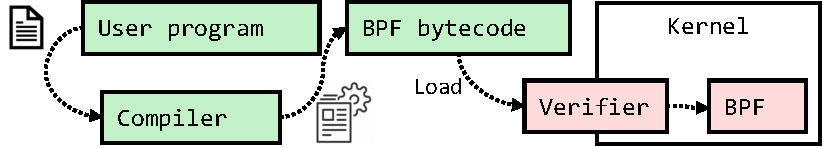
\includegraphics[width=1.0\linewidth]{figs/bpf_intro.pdf}
%%     \centering
%%     \vspace{-10pt}
%%     \caption{Overview of eBPF}
%%     \label{fig:ebpf}
%%     \vspace{-10pt}
%% \end{figure}

The safety properties checked by the eBPF verifier are generally
related to avoiding kernel crashes or hangs.  In eBPF, the verifier
uses a form of symbolic execution on the bytecode to examine all
possible executions to ensure safety.  It also performs limited
checks on the extension's
interactions with the kernel through {\em
  helper functions}.
We characterize these verifier
checks as ensuring the following conceptual properties of the
extension:
\begin{itemize}
\item {\bf Memory Safety:} Extensions can only access memory that is
  provided to them through explicit context arguments or kernel
  interfaces, (e.g., helper functions).  This prevents kernel crashes
  through NULL pointer dereference or corruption of kernel data
  structures.
\item {\bf Type Safety:} When accessing data in memory, the extension must use
  the correct type of the data. This helps avoid misinterpretation of the data
  or memory corruptions.
% When invoking kernel interfaces, the
%   extension must supply arguments of the appropriate type.  This helps
%   avoid kernel crashes in helper functions.
\item {\bf Resource Safety:} When gaining access to kernel objects
  (e.g., lock, allocated memory, etc.) through helper function,
  extensions must subsequently invoke the appropriate release
  interface on the object before completion.  This prevents memory
  leaks or deadlocks that can hang or crash the kernel.
\item {\bf Runtime Safety:} Extensions must terminate. This prevents
  infinite loops that hang the kernel indefinitely.
\item {\bf Undefined Behavior Elimination:} Extensions must never
  exhibit undefined behavior, including integer errors (e.g.,
  overflow, divide by zero, etc.). This prevents runtime kernel
  crashes.
\item {\bf Stack safety:} A unique safety requirement for kernel exntensions.
  Extension must not overflow the limited kernel stack.
  Failing to do so risks kernel crashes or kernel memory corruption.
\end{itemize}

This notion of safety in eBPF lowers the barrier to entry and trust
required for system administrators to install an extension into a
production system.  However, there are ongoing debates in
industry~\cite{reconsider-unpriv-ebpf-lwn,seccomp-ebpf-lwn,ebpf-sec-lwn} and
academia~\cite{untenableVerification} about the quality of eBPF's
safety guarantees and in what circumstances they can be relied on.
Here we specify the safety model and expectations for safety of kernel
extensions for the scope of this paper.

\paragraph{Safety model:} We assume that extensions are installed by a system administrator with
root privileges on the system.  Extensions are written by well-meaning
but imperfect developers and thus may contain programming mistakes.
We assume that the extension is not actively malicious.  So called
``guarantees'' of safety therefore consist of the best-effort catching
of common mistakes.  While some in the community may be interested in
exploring stronger notions of safety~\cite{reconsider-unpriv-ebpf-lwn,seccomp-ebpf-lwn,ebpf-sec-lwn,jia2023},
we note that this definition of safety is consistent with the current
eBPF ecosystem, where actively malicious extension writers can crash
or hang the
system~\cite{untenableVerification,ebpf-stackoverflow,ebpf-termination}
(e.g., via helper functions), but the verifier prevents obvious
mistakes (e.g., dereferencing a NULL pointer).

\section{The eBPF Programmer Gap}
\label{sec:motivation}

\begin{figure}
    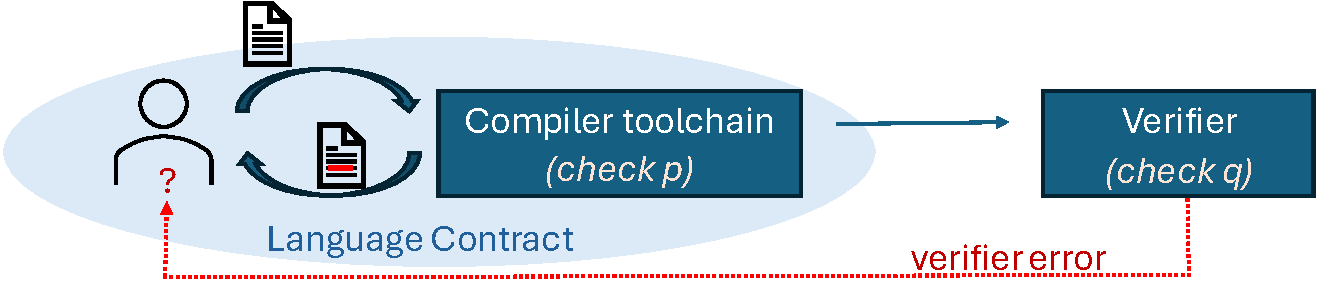
\includegraphics[width=1.0\linewidth]{figs/gap-crop.pdf}
    \centering
    \vspace{-10pt}
    \caption{The Language/Verifier Gap}
    \label{fig:gap}
    \vspace{-10pt}
\end{figure}


While eBPF verification is important for program safety, the eBPF verifier
    places additional constraints on programs, which results in usability challenges.
The core of the problem is a large gap between the programmer and the
    verifier.
Typical eBPF development involves implementing programs in a high-level
    programming language (e.g., C, Rust) and compiling to eBPF bytecode.
Developers agree to a contract with the high-level language, which is
    enforced by the compiler.
When a program fails to compile, the developer will get a message with
    hints about where they violated
    the contract with the programming language.
If, however, a program fails to pass the verifier it is harder for the programmer
    to understand why the program failed and how to fix it because the compiler
    and verifier do not pass information about program safety to each other.
%\mvle{not clear why it is hard for the programmer to understand verification failure messages.
%Is it because what is being verified is not the same program being written and not the
%same semantics being checked at the higher-level language?}

In order to quantify the impact of this gap,
    we analyzed commit messages from popular eBPF projects to see how programmers fix
    eBPF programs that fail to verify.
From the commit messages, we created a set of categories of fixes.
In the rest of this section we will describe our methodology and categorization, walk through some illustrative examples, and describe the key high level takeaways.
We find that the programmer gap as described exists, and that it makes the eBPF system less usable through the need for unintuitive programmer workarounds.
%\milo{Reword this last sentence}

%Additionally, we describe two fundamental reasons for the programmer gap.
%\milo{succinctly say them here.}



%At the same time, the verifier has a set of properties that it ensures are maintained for each program, such as memory safety.
%The verifier will reject programs that do not meet these properties.
%The compiler does not know the set of properties that the eBPF verifier checks, which
%    introduces a gap between the compiler and the verifier, and, by extension, the programmer and the verifier.
%
%The problem is compounded by the fact that the verifier operates on code that has undergone
%    translation from a high-level language into eBPF bytecode.
%The cause of verifier rejections may unrelated to the code the programmer wrote and instead
%    be a result of bugs anywhere along the toolchain.
%The verifier is also a moving target, with different versions having different constraints
%    and different completeness guarantees.
%As a result, eBPF developers often have to wrestle with the in-kernel verifier
%    to allow safe programs they write to pass.
%This can manifest itself in needing to write arcane expressions to please the
%    verifier, or by completely restructuring semantically correct and safe code.

%The compiler does not know the set of properties that the eBPF verifier checks, which makes it more difficult for developers to know if their program will run until they run the verifier.

%This binds developers with a contract not only with the high-level language
%    that is enforced by the compiler or interpreter, but also with the eBPF
%    verifier, where the specifications are not clear. \mvle{I don't it's an issue with specification. it's partly due to going from a turing-complete language to turing-incomplete. I think we should bulletize these challenges. 1. semantic gap (turing complete -> turing-incomplete, 2. difficult to debug due to many levels of translation, 3. compiler optimizations that are incompatible with verifier, 4. specification for verifier changes across kernel versions, 5. ?}
%Developers have a contract with the programming language that is enforced by the compiler of interpreter.
%The programmer also has a contract with the eBPF verifier, but the specifics are unclear.
%At the same time, because source code goes through a translation to eBPF
%    bytecode before verification, it is often difficult to map the verifier
%    error back to source code.
%Source code goes through a translation to eBPF bytecode before it is verified, which makes mapping the output of the verifier back to the code the programmer wrote difficult.

%To better understand this gap and the kinds of usability issues eBPF
%    developers face, we carried out an analysis on existing eBPF projects and
%    past research literature.
%We carried out an analysis of existing eBPF projects and research papers to better understand this gap and the kinds of verifier issues the eBPF developers face.
% eBPF developers often have to wrestle with the in-kernel verifier to allow the programs they write to pass.
% This can manifest itself in needing to write arcane expressions to please the verifier.
%We categorize the solutions that programmers need to implement in order to pass the verifier to get a clearer picture of the usability challenges that the current eBPF system has.

\subsection{Methodology}
To collect data, we searched through the git commit logs of Cilium~\cite{cilium}, Aya-rs~\cite{aya-rs}, and
    Katran~\cite{katran}, which are mature, widely-used eBPF projects, for instances of
    keywords: "error", "reject", "rejects", "issue", and "verifier."
For each commit log that matched, we manually inspected and classified the commit.
In total, we collected 216 commit messages containing the above keywords, of which we decided that 73 of them were actually about verifier complaints.
In addition, we included two issues raised in the BMC~\cite{BMC} and Electrode~\cite{Electrode} papers as examples when appropriate.

%88\% of commit messages found were from the Cilium repository.
%Cilium is a mature project that makes extensive use of eBPF as a core part of its architecture.
%Cilium represents a representative set of challenges for large projects with complex eBPF code bases.
%\jinghao{Is this paragraph necessary?}

%To classify the commits into categories, we read each of the commit messages and examined
%    their source code changes.
%Some categories were clear to see and are well documented in the literature (i.e. restructuring eBPF programs), while other categories were more subtle.
%We created a qualitative analysis of many of the kinds of fixes that are used when writing and verifying eBPF programs.

%The categorizations that we created are not necessarily mutually exclusive.
%We started with a large set of smaller categories, and then combined categories to
%    create larger categories that represented classes of fixes, as well as picking out
%    common patterns that are representative.

\subsection{Categorization Overview}

\begin{table}[t]
    \small
    \centering
    \begin{tabular}{lc}%{|p{6cm}|p{1cm}|}
        \toprule
        \textbf{Category} & \textbf{Count} \\
        \midrule
        Restructure eBPF program for verifier & 27 \\           % #2
        Change source code to fix LLVM codegen & 22 \\          % #1
        Add specific code to pass verifier & 17 \\              % #3
        Implement kernel-version-specific fixes & 9 \\          % #4
        %Add "pruning checkpoints" to reduce complexity & 7 \\   % #5
        % Move to section restructure bpf program for verifier
        % moved to #2 Refactor code because of lack of expressiveness & 2 \\
        % moved to #2 Split eBPF programs for complexity & 13 \\
        % moved to #2 Refactor code to reduce complexity & 5 \\
        % moved to #3 Inline functions to pass verifier & 6 \\
        % moved to #3 Explicitly teach the verifier information & 6 \\
        % moved to #3 Add bounds to a helping function & 3 \\
        % moved to #3 Add a specific implementation of a helping function & 2 \\
        \bottomrule
    \end{tabular}
    \caption{Table of common verifier fixes} %\mvle{we should rename these categories. These don't sound like verifier problems but actions done to overcome verfier issues.} \milo{These were meant to be fixes not problems, but the table title was a hold-over from before}}
    \vspace{-20pt}
    \label{fig:commit-table}
\end{table}

Our analysis classifies the commits into four categories.
Each category represents a class of techniques that developers used to make their programs pass the verifier.
Table~\ref{fig:commit-table} summarizes the results of our analysis.

%\jinghao{
%Some comments on the table: it is not immediately clear on what exactly
%    the developers are doing for some of the categories, especially the last
%    3. (btw, should it be ``helper functions'' or ``helping functions'').
%At the same time, the categories do not seem to be mutually exclusive,
%    e.g., ``Split eBPF programs for complexity'' vs.
%    ``Refactor code to reduce complexity''.
%We should be clear whether the categories are overlapping.
%}

The composition of the categories makes it clear that developers have to change their code in particular ways to get it to pass the verifier.
It also demonstrates how difficult it can be to reason about the results of the verifier.

There are two basic reasons an eBPF program can fail to verify. %for several reasons.
The first reason is when the program is unsafe, and the verifier correctly rejects it.
The second reason is when a program is actually safe but the verifier is overly conservative
in how it checks the program, and thus rejects it.
When the verifier rejects a safe program, it is up to the developer to find a way to show the verifier that the program actually is safe.
Each of the commits we categorized captured cases where the original code was safe, but the
    verifier rejected it.
The classes of solution employed are different ways that developers use to make sure the verifier accepts their programs.
%\jinghao{This paragraph is reptitative given the preamable, I think what is
%    missing here is an overview of the finding from our study (i.e. beef up the
%    previous paragraph)}

\subsection{Category Representative Examples}
To better explain our categorization, we now walk through representative examples for each category.

\subsubsection{Restructure eBPF program for verifier}
\label{motivation:restructure}
A big theme across the commits we found was the need to explicitly restructure eBPF programs to pass the verifier.
We identified two main techniques for restructuring programs: splitting eBPF programs into smaller programs, and refactoring programs to reduce verification complexity and overcome expressiveness limits.
We now use BMC\cite{BMC} as a representative example for this category.

%\begin{enumerate}
%    \item Split eBPF programs into smaller subprograms
%    %\item General refactoring to reduce verifier complexity or bypass expressiveness limits
%    \item Refactor eBPF programs to reduce complexity or bypass expressiveness limits
%\end{enumerate}

%TODO: Commented out to see if BMC can do all this
%\noindent\textbf{Splitting eBPF Programs}:
%A well documented technique to decrease overall eBPF program complexity is to use eBPF tail calls to split programs into several smaller subprograms that can be verified independently.
%The idea behind the split is that if each individual piece is verified to be safe, then the verifier itself would have verified the entire program if it could check enough instructions.
%Prior works like BPF Memcached Cache (BMC)~\cite{BMC} and Electrode~\cite{Electrode} utilize this technique in order to pass the verifier.
%BMC is split into seven different eBPF programs, and Electrode is split into six different eBPF programs.
%Both of these projects use around 500 lines of C code to program the eBPF programs.
%
%Modularity is good when programmers can split their code up into logical units, however due to the constraints of the verifier, they must split their code to match the verifier.
%In this case, we are left with program fragments which do not represent an individual unit, which makes the code harder to read and write.
%This compounds with the fact that the compiler has no notion of these limits.
%The compiler would happily compile both the split versions of code and the unified version of code, however only one set of code would pass the verifier.
%Additionally, it is not necessarily trivial to split these functions because all safety checks need to be made in each subfunction in order for them to be independently verified.
%%\jinghao{Why is this the case?
%%I think there are 2 cases, one is that the developers can just
%%split the program at the logical boundaries so that they actually get the
%%modularity; the other case is that they simply cannot split the program at these
%%boundaries and have to break it into fragments, I think this is what we are
%%arguing for and we have already seen in the case of BMC where they have to
%%keep a ``parse context'' across tail calls.}
%
%
%% The BMC has many places where for loops are nested into different ifs.
%% And, due to the limitations of C, many operations do not have built-in functions
%%     that can be used directly.
%
%\noindent\textbf{Refactoring Code}:
%\mvle{isn't splitting code a form of refactoring?}
%Code may also need to be refactored to reduce its complexity, or to work around limitations in the verifier.
%
%An example of refactoring to reduce complexity is found in a Cilium commit that involved changing how the code handled IPv4 fragmentation.
%As seen in Figure~\ref{fig:refactor-fix} the code used an \texttt{\#ifdef} with a default behavior.
%If \texttt{ENABLE\_IPV4\_FRAGMENTS} was enabled, then the code would be compiled with both the \texttt{ipv4\_handle\_fragment} call and the \texttt{ctx\_load\_bytes} call.
%%If the packet was a fragment, then the \texttt{ipv4\_handle\_fragment} call would have completed the loading of bytes, and the additional call would have been redundent.
%%\jinghao{I recommend removing this last sentence. It makes it sounds like a
%%good thing that developers have to remove some redundent code.}
%
%This design however, caused the program to fail verification as it went over the maximum checked instruction limit.
%The code was then refactored to change the \texttt{\#ifdef} and the underlying function.
%This change does not change the safety properties of the program, but it was still needed to verify the program.
%
%\begin{figure}
%    \lstinputlisting[language=myC]{./snippets/s2-refactor.c}
%    \caption{Refactor for Code Complexity}
%    \label{fig:refactor-fix}
%\end{figure}
%
%Refactoring is also used by programmers to overcome limitations in the verifier to recognize safe code due to the way the program is specifically expressed.
%An example of such a case is found in the Cilium project.
%%We found an example of refactoring for expressiveness in the Cilium project.
%To implement segment routing header support, they needed to include code to jump back to the beginning of the IP header parsing code while already inside the IP header parsing code.
%This would cause a back-edge which gets incorrectly labeled as an infinite loop and the verifier fails.
%Figure~\ref{fig:switch} shows their solution which involved creating a switch statement inside of a switch statement which then jumps ahead to the other code in the outer switch statement.
%The changes required increase the complexity of the source code without changing the semantics.
%
%\begin{figure}
%    \lstinputlisting[language=myC]{./snippets/s2-switch.c}
%    \caption{Refactor for Expressiveness}
%    \label{fig:switch}
%\end{figure}
%% TODO: End Comment

\noindent\textbf{BMC Example}:
%BMC had to split eBPF programs into smaller subprograms, and refactor code for verification complexity 
%    in order to immplement 
%Both of these verifier fixes were needed to implement BMC, an in-kernel cache for Memcached
%    based on eBPF.
%BMC stores recently queried key-value pairs in an eBPF map (i.e. the cache) to
%    accelerate the processing of GET requests to the Memcached server.
% The map that serves as the cache is managed by eBPF programs, which implements
%     the lookup and update logics.impl:ctx-converison

Implementation-wise, BMC is much more complicated
    compared to other common eBPF use cases.
In order to pass the verifier, it has to be split into seven
    eBPF programs that use eBPF tail calls to transfer control to each other. 
%    to reduce verification complexity.
Ideally, only two eBPF programs are required, one at ingress and one at egress.
Unfortunately, splitting eBPF programs for the verifier leaves program fragments 
    that are not self-contained and
    BMC sometimes has to pass computation states across tail calls, by using a map.
%BMC utilizes a map to pass current computation state across tail calls.
%This is because tail-called eBPF programs can only take the regular eBPF
 %   context as arguments.
The computation state is stored before the tail call and reloaded afterwards.

%A similar problem also presents when processing the incoming packet data, where
%    the authors had to bound data size to simplify verification of loops.
%\mvle{verifier complexity or program complexity?}
BMC suffers from verification complexity in its cache invalidation function,
    as examplified by its cache invalidation logic. % shown in Figure~\ref{fig:bmc-code}.
\mvle{what's bad about verification complexity? does it lead to verification failure?}
The complexity is exacerbated by introducing two additional variables to track
    the state of the key and the SET command.
To address the verification complexity,
    the cache invalidation code employs \texttt{for} loops with cumbersome
    condition checks, and is further complicated by the nesting of multiple
    \texttt{if} statements.
Without these checks, the program produces an excessive number of jump instructions,
    leading to verification failure.
We discuss this in more depth in our case study for BMC
    (\S\ref{eval:bmc-case-study}).

% \jinghao{Let me know if removing this makes sense: ``and the end of packet''.}
%Such complex checks are intentionally designed to pass the
%    verifier.
% the verifier to reject loading the program.
%This approach significantly increase the programming burden
%    of BMC, while at the same time leads to readability issues in some places
%    regarding the intended functionality.
%% \jinghao{One or two sentence explain why conditions are needed for
%%     verification, based on our experiment on removing one of these.}
%% This situations is a prevalent pattern within the BMC structure, which is
%Such pattern is prevalent in the BMC implementation, which is
%%    notably observed within the functions \texttt{bmc\_hash\_keys\_main}
%%    and \texttt{bmc\_write\_reply\_main}.
%    notably also present in the code that hashes the Memcached key and drafts the reply.
%In the initial design of \projname{}-BMC, the underlying assumption was that
%    we should follow the logic of BMC.
%But the cache invalidation function Figure~\ref{fig:bmc-code} in BMC employs
%    \texttt{for} loops with cumbersome condition checks, and is further
%    complicated by the nesting of multiple \texttt{if} statements.

%Another example that the verifier creates programming burden for BMC is its
%    instruction count limit.
%\mvle{seems to repeat the "implementation-wise para}
%% Due to the instruction count limitation imposed on each eBPF program,
%%     BMC has to adapt a strategy of creating seven seperated eBPF
%%     programs to function as a Memcached cache layer.
%Due this limit, BMC has to be split into seven separated eBPF program, while
%    ideally only two are required (at egress and ingress hooks).
%% To pass messages across tail calls, BMC employed a specific struct
%%     called \texttt{parsing\_context} for storing the metadata and
%%     put the struct in the map named \texttt{map\_parsing\_context}.
%\mvle{I think this BMC section can be shortened significantly as it feels all the points
%have already been made and these are just additional examples.}

Both of these techniques are required for BMC to pass the eBPF verifier, but they
    increase the programming burden, and produce code that is more difficult
    to maintain.
The fixes implemented are not immediately apparent or trivial to implement, as
    exemplified by the complex branch conditions, and state restoring through maps.
Fighting with the verifier made the implementation of BMC much more difficult then
    it needed to be because of the gap between the programmer and the verifier.

% \begin{figure}[t]
%     \lstinputlisting[language=myC]{./snippets/s6-bmc.c}
%     \vspace{-10pt}
%     \caption{Packet parsing code for cache invalidation in BMC}
%     \label{fig:bmc-code}
%     \vspace{-10pt}
% \end{figure}

\subsubsection{Change Source Code to Fix LLVM Codegen}
\label{motivation:llvm-codegen}
The LLVM compiler translates eBPF programs written in high-level languages into eBPF bytecode.
We found that in certain cases, LLVM would generate eBPF bytecode that would cause the program to fail verification.
One issue found by Cilium was that LLVM may generate 32-bit assignments for
    accessing the \texttt{ctx->data}, \texttt{ctx->data\_end}, and \texttt{ctx->data\_meta} fields.
The LLVM compiler thought that the \texttt{data} fields were 32-bit values rather than 64-bit pointers as
    a result of the information hiding technique that
    eBPF employs.
The kernel exports a limited context interface to extension programs that is then rewritten in the verifier.
%The kernel exports a context interface to extension programs with only
%    the fields that they may need, and at verification time all accesses to
%    these fields are rewritten by the verifier to the actual kernel-internal
%    data structure.
The above fields are defined as 32-bit integers in the exported interface and
    the LLVM compiler does not know that this gets rewritten by the verifier into 64-bit pointers.

%Since the \texttt{data} field is defined as a 32-bit integer in the dummy
%    interface the kernel exports, the compiler, which does not see the
%    subsequent rewriting and kernel-internal definition, treats it as a real
%    32-bit integer and performs code generation, even though \texttt{data} is
%    actually a 64-bit pointer.

%Figure~\ref{fig:inline-error} shows the verifier losing track of the packer pointer.
%At instruction 3, R6 gets the value of R9, but this is a 32-bit assignment, as indicated by the `w' prefix.
%Then in the next line we see that R6 has type `inv' which is a scalar value, and \emph{not} a pointer to a packet showing that the verifier lost track of the type of R6.

%The \texttt{data} field is

To fix the problem, Cilium implemented access to \texttt{data} fields using inline assembly code. %shown in Figure~\ref{fig:inline-asm}.
LLVM no longer generates the problematic 32-bit assignments as an optimization because it cannot optimize the
    inlined assembly.
The verifier can then treat the register as a packet pointer, rather than a scalar.
%\jinghao{It is actually not too clear how this fixes the problem -- for
%specifically how is the generated code different?}
%\jinghao{can we be more specific on the BPF opcode (e.g., load/store) of the
%    assignment as in Figure~\ref{fig:inline-asm}}

Other commits use the \texttt{volatile} to prevent LLVM from performing other optimizations
    that cause the verifier to reject the program.

These workarounds allow the eBPF program to pass the verifier.
It is clear that they expose usability issues of the verifier.
The LLVM compiler is unaware of what the verifier checks and any modifications the verifier does to extension programs.
Programmers must then know low level details about the eBPF system and LLVM bytecode generation in order to fix verifier issues for safe programs.


%\begin{figure}
%    \lstinputlisting[language=myBPF]{./snippets/s2-codegen-error.c}
%    \caption{Verifier log for LLVM generated 32-bit assignment}
%    \label{fig:inline-error}
%\end{figure}

%\begin{figure}
%    \lstinputlisting[language=myC]{./snippets/s2-inline-asm.c}
%    \caption{Inline asm to access fields}
%    \label{fig:inline-asm}
%\end{figure}



\subsubsection{Add specific code to pass verifier}
\label{motivation:add-code}
Another common fix for verifier complaints involves adding specific code to please
    the verifier.

%This can involve several kinds of new specific code:
%
%\begin{enumerate}
%    \item Adding inline functions
%    \item Teaching the verifier information
%    \item Implementing functions in a specific way
%\end{enumerate}

\noindent\textbf{Inlining Functions to Pass Verifier}:
The verifier can lose track of information depending on how eBPF programs are structured.
One fix for this is to inline functions for implementing functionality.
It is not always clear what code needs to be made into an inlined function for the verifier
    which makes eBPF less usable.

\begin{figure}
    \lstinputlisting[language=myC]{./snippets/s2-goto.c}
    \vspace{-10pt}
    \caption{Goto transformed to inline function}
    \vspace{-10pt}
    \label{fig:inline-fig}
\end{figure}

%\begin{figure}
%    \begin{lstlisting}[language=myC]
%policy_check_entry:
%	account(ctx, policy);
%
%	if (unlikely(policy->deny))
%		return DROP_POLICY_DENY;
%
%	*proxy_port = policy->proxy_port;
%	if (unlikely(policy->auth_type)) {
%		if (ext_err)
%			*ext_err = (__s8)policy->auth_type;
%		return DROP_POLICY_AUTH_REQUIRED;
%	}
%	return CTX_ACT_OK;
%}
%    \end{lstlisting}
%    \caption{Block of code reached after a goto}
%    \label{fig:inline-fig}
%\end{figure}

For example, in Cilium, code that performed policy checks used goto statements to prevent code duplication.
As seen in Figure~\ref{fig:inline-fig} the \texttt{policy} variable could be used to refer to \texttt{policy} or \texttt{l4policy} before jumping to the checking logic.
This caused the verifier to reject the program because it lost track of what the \texttt{policy} variable referred to.
The developers fixed this by converting the policy check logic from a labeled block of code reached by a \texttt{goto}, to an inline function.
The original structure of the code before was valid and correct, but it failed to pass the verifier.
%In response to this, the developers had to figure out a workaround to make their valid code pass.

%The developers made this code general across two cases by reassigning the value of policy depending on what the input was before jumping to the common code.
%This pattern caused the verifier to lose information about what the variable \{policy{ was referring to.
%The fix was to convert this common code into an inlined function.
%\jinghao{
%It is hard to see why this is a problem, especially when you say ``Doing this
%    helps to keep functionality separate from the programmers perspective,
%    while allowing the verifier to see all the code at the same time''.
%I think we need something similar to the previous cases where we explicitly
%    discuss why it is bad.
%}

\noindent\textbf{Explicitly teaching the verifier information}
%An example of explicitly teaching the verifier information can be found in the Aya-rs project.
%As part of their library, Aya contains functions to help log information.
%Throughout the project they have an upper bound on the size of the log buffer.
%In a write string function they needed to add an explicit check on the size of the length of the string against the log buffer max size.
We found an example in Cilium where the developer needed to explicitly teach the verifier
    information.
The verifier lost track of the value of \texttt{nh\_params.nh\_family}, which caused it to reject the program.
In Figure~\ref{fig:teach-verifier}, we can see that the developers needed to slightly change the code in order to ensure the verifier knew what the value was.
The original code was fully safe, but the verifier rejected it.
The required fix is unintuitive, which makes it less usable.

\begin{figure}
    \lstinputlisting[language=myC]{./snippets/s2-teach.c}
    \vspace{-10pt}
    \caption{Teaching the verifier info}
    \vspace{-10pt}
    \label{fig:teach-verifier}
\end{figure}

\noindent\textbf{Reimplementing functions}
%\mvle{can we summarize what is this "specific" way?}
We found examples of this in both Cilium and Aya-rs.
Both of these projects found uses for the functions \texttt{memset} and \texttt{memcpy}, but they had to provide their own versions of them.
Aya-rs took the approach of writing a simple version that looped over the data safely, while Cilium used a much more complicated approach, a portion of which is shown in Figure~\ref{fig:cilium-memcpy}.
Both of these code snippets were designed to pass the verifier.
Rather than use a standard library function, eBPF programmers have to reimplement the required functionality.
This makes developing eBPF programs more difficult, especially when the implementation of
    required functions is nontrivial and has to fight the verifier.

From these examples it is clear that programmers need to add code to their
    eBPF extensions to please the verifier.
The needed code is nontrivial, and the programmer receives little help from the verifier to track down
    the problem.
The compiler provides no help at all, due to the \gap{}.
%\begin{figure}
%    \begin{lstlisting}[language=rust]
%#[no_mangle]
%pub unsafe extern "C" fn memcpy(dest: *mut u8, src: *mut u8, n: usize) {
%    let dest_base = dest as usize;
%    let src_base = src as usize;
%    for i in 0..n {
%        *((dest_base + i) as *mut u8) = *((src_base + i) as *mut u8);
%    }
%}
%    \end{lstlisting}
%    \caption{Simple and specific implementation of memcpy}
%    \label{fig:aya-memcpy}
%\end{figure}

\begin{figure}
    \lstinputlisting[language=myC]{./snippets/s2-cilium-memcpy.c}
    \vspace{-10pt}
    \caption{Memcpy implementation in Cilium}
    \vspace{-10pt}
    \label{fig:cilium-memcpy}
\end{figure}

\subsubsection{Implement kernel-version-specific fixes}
\label{motivation:kernel-version}
Different kernel versions may have different versions of the eBPF verifier, each with different sets of bugs.
To maintain compatibility between these versions, developers have to change code to account for the differences.
A good example of this is found in Cilium.
%The verifier failed the program with the message shown in Figure~\ref{fig:kernel-version}.
The verifier rejected a program because it saw an invalid access of a context pointer, even though
    it was a valid access.
The specific scenario is an instance of a known verifier bug that has been fixed, but the fix is not present in all kernel versions.
Cilium developers had to implement a simple, but precise fix to ensure that the program would verify on all extensions.
As shown in Figure~\ref{fig:kernel-version-code} the fix needed was to move line 7 to line 1 before the block of code.
Version mismatches make eBPF much harder to use as they are decoupled.
We discuss this further in \S\ref{discussion:versions}.

%\begin{figure}
%    \begin{lstlisting}[language=myBPF]
%1411: (bf) r1 = r9
%1412: (07) r1 += 48
%1413: (67) r2 <<= 16
%1414: (47) r2 |= 512
%1415: (63) *(u32 *)(r1 +0) = r2
%; dereference of modified ctx ptr R1 off=48+0,
%; ctx+const is allowed, ctx+const+const is not
%    \end{lstlisting}
%    \caption{Verifier output showing error}
%    \label{fig:kernel-version}
%\end{figure}

\begin{figure}
    \lstinputlisting[language=myC]{./snippets/s2-kernel-version.c}
    \vspace{-10pt}
    \caption{Kernel version specific fix}
    \vspace{-5pt}
    \label{fig:kernel-version-code}
\end{figure}

%\subsubsection{Add Pruning Checkpoints}
%\label{motivation:checkpoint}
%Another common fix that Cilium implemented was to introduce a pseudo-helper function \texttt{relax\_verifier}.
%The purpose of this helper is to provide a checkpoint for the verifier to use when doing state pruning.
%All the function does is call a kernel helper function, which then introduces a new state pruning checkpoint.
%%\jinghao{Can we put more information here on this helper? It would be great
%%to show that the helper itself is complicated and developers have to insert it
%%at random places.}
%%\jinghao{My understanding is that this calls a \textit{kernel helper} so that the
%%state is reset?}
%In some cases doing so significantly decreases the complexity of eBPF programs.
%In one commit, doing so reduced the number of instructions checked from 62,569 to 49,669.
%This is more significant on older kernel versions which have a much smaller upper limit to the number of instructions the eBPF verifier could check.
%\jinghao{It now seems to me that this belongs to \S\ref{motivation:restructure}.}
%\milo{I don't think so because the state pruning knowledge is more obscure, so needing to use it is harder than refactoring. i.e. A dev may know that their loops can't be too complicated, but they may not know anything about verifier internal state pruning? It also does not really change the structure (this is intentional)}
%
%With no assistance, programmers are required to have knowledge of low-level
%    internal details of the eBPF verifier, and then implement fixes that
%    make use of this knowledge.
%Having to make this change harms the usability of eBPF.


\subsection{Analysis Takeaways}
From our analysis, we believe that there are serious usability challenges in the
    existing eBPF system that stem from a large \gap{}. %gap between programmer and verifier.
The categories of verifier workaround that we found are direct indicators of this problem.
eBPF programmers have to implement arcane fixes and change their mental model of
    programming to meet the constraints of the verifier without any compiler assistance.
If an eBPF program fails to verify there is not always a clear reason why that was the case, e.g.,
it could be that a programmer's source code was completely safe, but LLVM generated code that the verifier did not understand.
To programmers, a successful compilation should indicate something about the success of their code, but in the eBPF system that is not the case.
This gap is fundamental to the eBPF system.
A system that closes this gap by moving the verifier and the compiler closer together may be able to avoid the challenges discovered in the existing eBPF system, while still ensuring program safety.
% \jinghao{would be interesting to talk about saving/reloading computation
%     context across tail calls}

%Different kernel versions have different verifiers with different constraints
%    and different properties that they check.
%There would have to be some way to fully expose the specifics of the verifier
%    back to the compiler to close the gap.

%\subsection{Mismatches Cause the Gap}
%In this section we examine two of the main causes of the programmer gap.
%The programmer gap is a consequence of two mismatches between the verifier and the compiler that arises due to the design of the eBPF system.
%    \begin{enumerate}
%        \item Version mismatches
%        \item Safety mismatches
%    \end{enumerate}

%\subsubsection{Version Mismatches}
%There are three sources of versioning that eBPF currently has, that may lead to issues.
%\begin{enumerate}
%    \item Kernel Interface
%    \item Verifier
%    \item Compiler
%\end{enumerate}
%
%Kernel interface version problems are resolved by the use of BTF and CO-RE in BPF.
%However, the version issues differences between the compiler and verifier are not dealt
%    with in any way.
%
%In the current eBPF system, the compiler and the verifier are decoupled.
%As development proceeds, implementation details about the compiler and verifier change.
%As seen in Table~\ref{fig:commit-table} there are examples of differences in implementation
%    between the LLVM compiler toolchain and the eBPF verifier breaking
%    program verification.
%Figure~\ref{fig:2comp1ver} shows a flowchart of how this might happen.
%
%Problems can also arise from different verifier versions.
%If an eBPF program verifies on one version, there is no guarantee that it verifies on a different version.
%Examples of this include backwards compatibility for features like loops.
%Figure~\ref{fig:1comp2ver} shows a flowchart of how this might happen.
%
%There is no way to fully resolve the issues of versioning in the eBPF system as
%    each component is a constantly moving target.
%Compilers will continue to evolve, just as the eBPF verifier will continue to evolve, and because they are decoupled, there will be places where they do not align.

%\begin{figure}
%    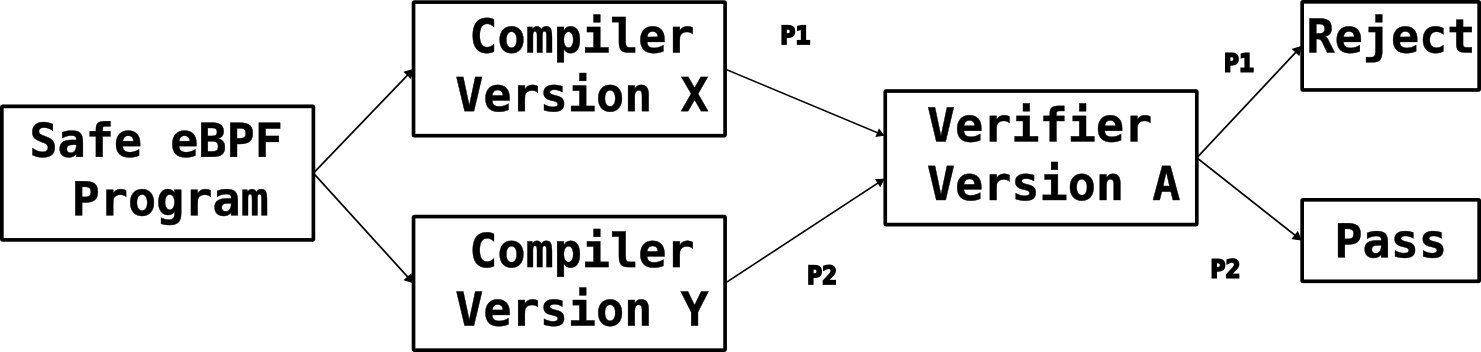
\includegraphics[width=1.0\linewidth]{figs/2comp1verifier}
%    \centering
%    \caption{Version issue between two compiler versions}
%    \label{fig:2comp1ver}
%\end{figure}
%
%\begin{figure}
%    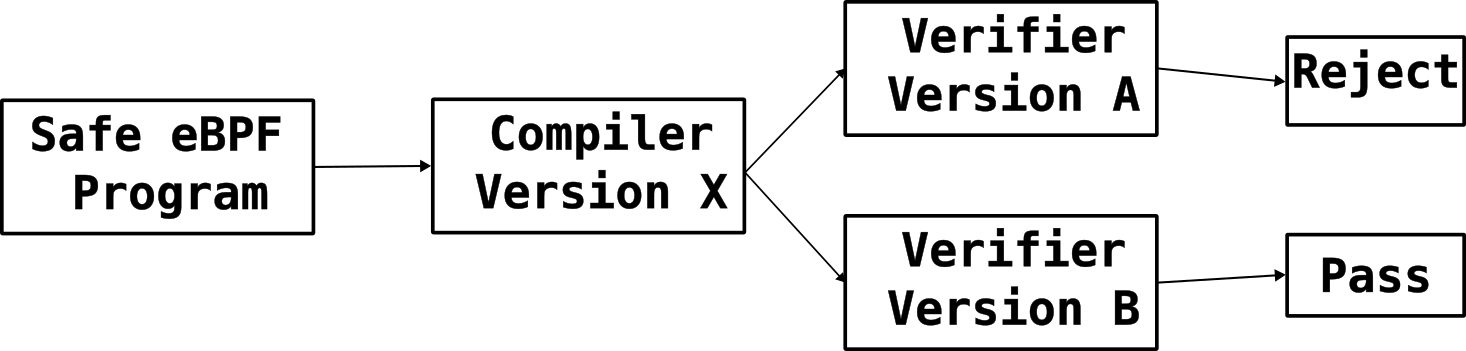
\includegraphics[width=1.0\linewidth]{figs/1comp2verifier}
%    \centering
%    \caption{Version issue between two verifier versions}
%    \label{fig:1comp2ver}
%\end{figure}





\section{Safety in \projname{}}
\label{sec:principle}

% \jinghao{\S\ref{sec:principle}: How to make it safe}

%\begin{itemize}
%    \item goal: expressive and safe (more expressive than and at least as safe
%        as eBPF)
%    \item Current problem of eBPF: the verifier
%    \item Idea: remove the verifier and use a safe language
%    \item the language should be Turing complete and at the same time low-level
%        enough to provide safety features.
%    \item We choose Rust as the implementation language.
%    \item The use of Rust automatically provides eexpresssiveness
%    \item We then show how a safety can be achieved for kernel extensions via
%        language-based safety from Rust.
%    \item how to ensure safety (high-level discussion, no implementation
%        details)
%        \begin{itemize}
%            \item builtin memory/control/type safety
%                \begin{itemize}
%                    \item generic and const-generic functions and slices to
%                        prevent OOB access
%                    \item Safe direct packet access for XDP programs
%                    \item Retired expressiveness kernel helpers (\jinghao{probably does not belong here})
%                \end{itemize}
%            \item RAII (e.g. lock, refcnt)
%            \item exception handling and stack unwinding
%                \begin{itemize}
%                    \item Needed because Rust itself has runtime checks (e.g.
%                        array OOB access)
%                    \item handle exceptional control flow
%                    \item clean up resources to achieve RAII under exceptional
%                        circumstances
%                \end{itemize}
%            \item runtime mechanism to support properties that are
%                (fundamentally) hard to check at compile time
%                \begin{itemize}
%                    \item program termination
%                    \item stack overflow protection
%                \end{itemize}
%        \end{itemize}
%\end{itemize}

% Some small things here and there
%
% - no clone impl for objects returned by RT crate to ensure uniqueness
% - difference between userspace Rust: there are things the compiler cannot see
%   e.g., we cannot have something like Mutex::get_mut in bpf_spinlock to
%   access a value w/o lock using the single-mutable-reference rule


The goal of \projname{} is to provide enhanced usability for kernel extensions,
    while ensuring safety of the extension programs.
In particular, we aim to make \projname{} more usable than eBPF and as safe.
As discussed in \S\ref{sec:motivation}, the current problem of usability of
    eBPF is the large \gap{}. % between the programer, who works on
    % high-level languages, and the verifier, which operates on compiled bytecode.
% Our insight is that both the needed expressiveness and safety can be obtained
%     from a safe programming language without the verifier.
Our insight is that by using a safe, high-level language that directly
    implements the required safety properties of kernel extensions, the need
    of the extra verification layer can be dropped, and thereby closing the
    \gap{}.
\mvle{not completely true tho since we need the runtime part for termination}

% Specifically, the language should have the following properties:
% \begin{itemize}
%     \item \textbf{Turing-complete}: This helps to satisfy the expressiveness
%         requirement.
%     \item \textbf{Safe}: The language should not be as permissive and
%         error-prone as unsafe languages like C.
%     \item \textbf{Low-level}: Being low-level helps the programs to better
%         model low-level kernel semantics and simplifies infrastructure needed
%         to support it.
% \end{itemize}

% \djw{background on Rust moves here}
% Need to talk about:
% - Language-based safety no undefined behavior in Rust.
% - Safe/unsafe Rust.
% - Popularity (also embraced by kernel)

\projname{} chooses Rust as the safe language for extension programs.
Rust is a system programming language that aims to provide
    \emph{language-based} safety, which promises programs to be free of
    \emph{undefined behaviors}.
The compiler both performs static analysis (e.g., lifetime and ownership
    models) and inserts dynamic checks (e.g. array bounds checks) in
    Rust programs to fulfill its safety promises.
To facilitate low-level code that may be hard to fit into its safety model (e.g.
    FFI calls), the language also provides \emph{unsafe} Rust, which is more
    permissive and provides a weaker safety guarantee, as opposed to
    \emph{safe} Rust.
Utilization of the language-based safety of Rust under kernel contexts has been
    explored by previous works~\cite{redleaf,theseus}, and is also incorporated
    into the Linux kernel~\cite{rust-for-linux-lwn}.
% This is because Rust happens to provide the desired properties -- its
%     language-based safety can be leveraged for safe kernel extensions without a
%     verifier.
In \projname{}, Rust provides either the desired properties directly or
    essential building blocks to ensure the important safety properties for
    kernel extensions (\S\ref{sec:background}).
% Here, we list the important safety properties
% (\jinghao{may need to move to \S\ref{sec:background}})
% \begin{itemize}
%     \item Memory safety
%     \item Type safety
%     \item Safe resource management
%     \item Exception-based runtime safety
%     \item Stack safety
%     \item Program termination
% \end{itemize}

% \jinghao{The runtime exception handling is not necessarily an independent one,
% it actually covers some of the type safety (arrays and slices does runtime
% checks that may trigger exceptions)}
\begin{figure}
    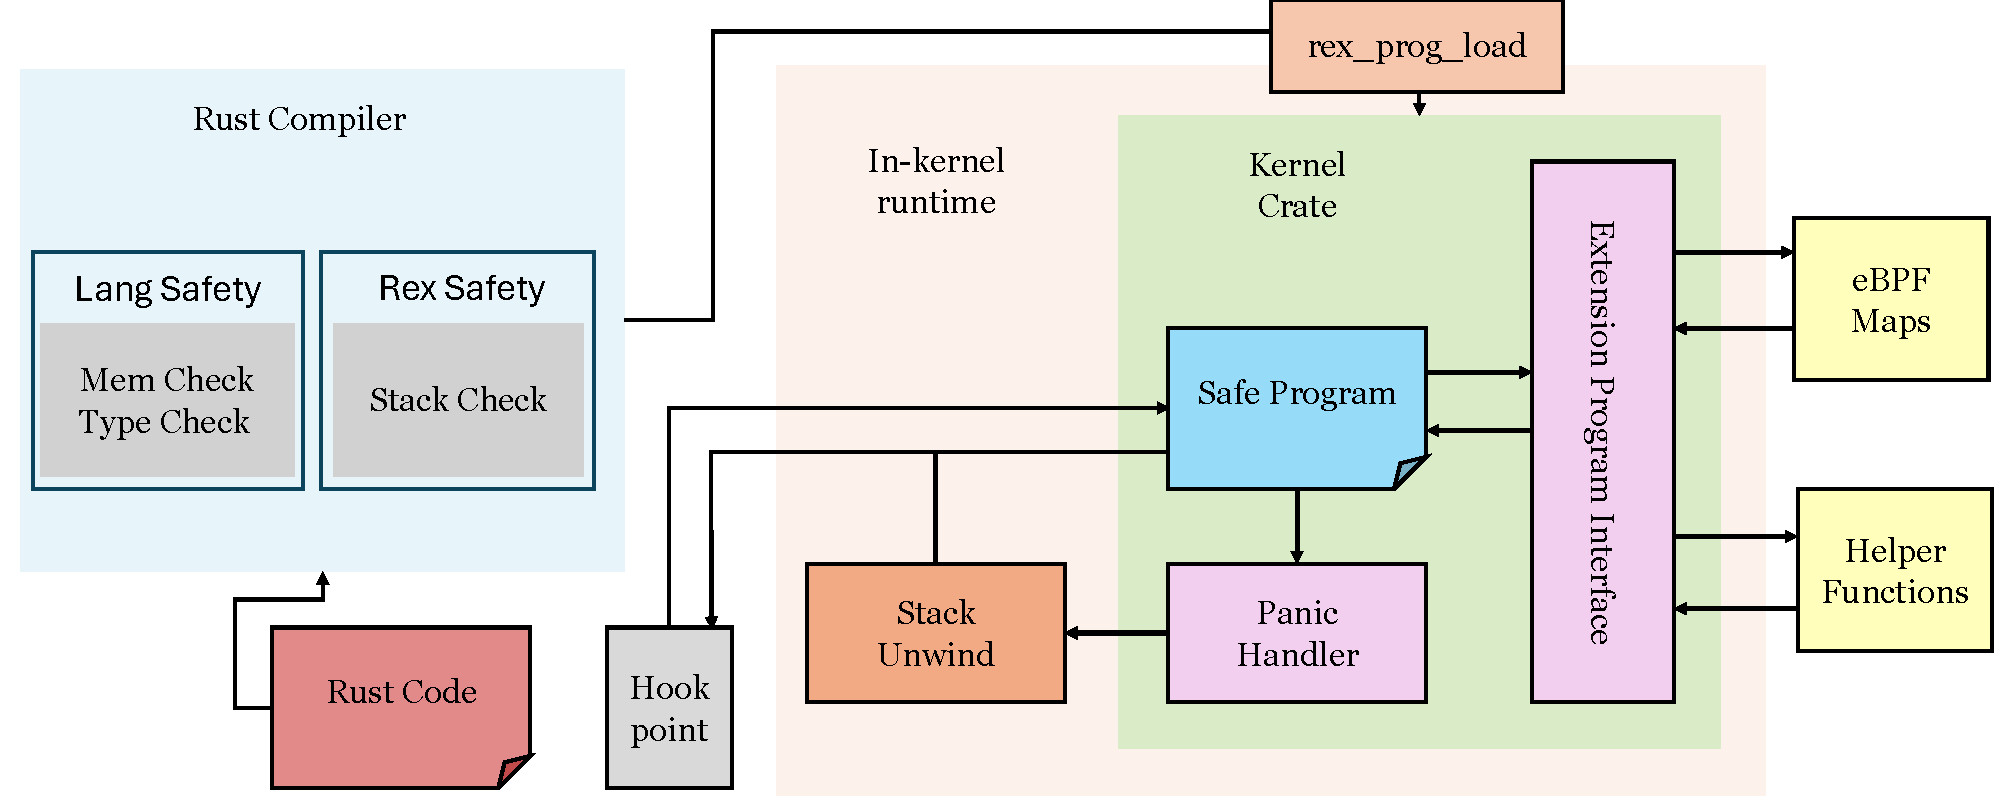
\includegraphics[width=1.0\linewidth]{figs/overview.pdf}
    \centering
    \vspace{-10pt}
    \caption{Overview of \projname{}}
    \label{fig:rex-overview}
    \vspace{-10pt}
\end{figure}

We now discuss how the language-based safety from Rust can be applied to the
    context of kernel extensions to provide a safe programming interface.
% While the use of Rust automatically provides expressiveness (as it is
%     Turing-complete), it does not supply the safety out-of-box, and the use of
%     Rust, especially unsafe Rust, can still exhibit undesired behaviors.
% We require all extension programs to be implemented \emph{only} in safe Rust.
% On top of that, we discuss how the safety properties from Rust can be leveraged
%     and applied to the context of kernel extensions to provide a safe
%     programming interface.
Figure~\ref{fig:rex-overview} provides an overview of the \projname{} framework.
The extension program is written strictly in \emph{safe} Rust.
It is compiled by the Rust compiler, which not only ensures safety properties
    in Rust but also runs a \projname{}-specific pass for kernel stack safety.
The program interacts with the kernel through a program interface implemented
    by the \projname{} \emph{kernel crate}.
The kernel crate contains a mixture of unsafe Rust code due to its role as a
    bridge between the extension program, which is expected to be checked for
    safety, and the unsafe but trusted kernel code.
It also provides a custom Rust panic handler to support panic-based runtime
    safety checks in Rust.
The program links with the kernel crate at compile time and runs in a
    light-weight runtime environment implemented in the kernel, which provides
    program termination and stack unwinding support.

\subsection{Memory safety}
\label{principle:memsafety}
Generally, kernel extensions are not allowed to access kernel memory.
However, there are frequent cases that an extension program needs to work on a
    shared buffer of data or a specific struct, and exchange data with the
    kernel.
% These regions of memory are accessed by both the program via helper functions
%     and the kernel.
% Rust provides powerful primitives that help to validate the memory is
%     accessed correctly.
There are usually two common patterns on how the memory is accessed, differing
    by the owner of the memory: 1) Memory owned by the extension program (e.g.,
    an on-stack buffer) is sent to the kernel through the helper function
    interface. 2) Memory owned by the kernel (e.g., an in-kernel struct) is
    accessed from the extension program. % direct packet access, map data ptr

In the first case, the extension program may allocate some memory on the stack
    and send it to the kernel for processing (e.g., asking kernel to fill a
    stack buffer with some data).
An unsafe memory access, for example, an out-of-bounds write to the on-stack
    buffer, could result in corruption of stack data and possibly trigger a
    kernel crash if the return address is overwritten to a non-present page.

For eBPF, the verifier validates the memory region with the size to make sure
    that both the kernel and the program do not make erroneous accesses.
For the memory buffers sent to the kernel through the helper function interface,
    the corresponding size is also sent as an argument to the helper.
The verifier, at program load time, checks to ensure that the size is exactly
    that of the memory buffer.
Then, at runtime, the kernel can operate on the buffer with the knowledge of
    its bounds, thereby avoid unsafe memory accesses.

In \projname{}, the strict type system of Rust already protects the program
    from making an unsafe access.
\projname{} leverages the generic programming feature of Rust to ensure the
    size sent through the helper function interface is always valid.
% In order to make sure that the size sent to the kernel is always correct, which
%     is vital for the correctness of memory access from the kernel, we leverage
%     the generic programming support of Rust.
For kernel helper functions that take in a
    program-supplied pointer and size, the \projname{} kernel crate creates an
    adaptor interface that parametrizes the type of the pointer as a generic
    type parameter.
The interface queries the size of the generic type from the compiler
    and invokes the kernel interface with this size as the argument.
Since Rust employs monomorphization~\cite{rustc-monomorphize}, the concrete
    type and its size is resolved at compile time, adding no runtime overhead.
In this way, the size is guaranteed to match the type statically and the
    kernel will never make an out-of-bound access.
This can work for not only scalar types, but array types as well: Rust
    also supports ``const generics'' that allows a constant to be used as a
    generic parameter, which can be used to encode the length of arrays.

In the second case, the kernel may provide the user program a pointer to
    kernel memory to perform direct access (e.g., access through eBPF map value
    pointers and packet pointers).
The user programs must not make an out-of-bound memory access for this
    kernel-owned region of memory, as doing so risks corrupting kernel data.

In eBPF, for accesses on pointers with a static size, e.g. map value pointers,
    as maps store the size of its value types, the verifier can independently
    verify the validity.
For pointers without a static size like packet data pointers, the verifier
    enforces programs to explicitly check for memory
    boundaries and to not make out-of-bound accesses.

In \projname{}, pointers with a static size are handled through the Rust type
    system, as the
    kernel map interface of \projname{} encodes the key and value types through
    generics.
The type system therefore forces the pointer to be a safe Rust reference of
    the particular type.
Pointers referring to a memory region without a static size are generally
    dynamic-sized buffers.
The \projname{} kernel crate abstracts such pointers into a Rust \emph{slice}
    with dynamic size.
Rust slice provides runtime bounds checks (\S\ref{principle:eh}), which allows
    the check to happen automatically without explicit handling from the
    extension program.

\subsection{Extended type safety}
Kernel extensions may contain certain paradigms that are beyond the safe
    type system of Rust.
One challenge is to allow extension programs to safely reinterpret the stream
    of bytes into useful data.
Such cases are notably found in networking use cases, where a program may need
    to extract the Ethernet header from a byte buffer in the packet.
Safety of these transformations is hard to reason about because they
    inevitably involve unsafe type casting.
% For example, a XDP program using direct packet access might need to extract
%     the ethernet header information from the bytes in the packet.

Currently, eBPF allows the program to freely interpret the packet data into
    other data types via pointer casting.
The verifier checks the casting and ensures that 1) the program does not make a
    pointer from scalar values and 2) the new type fits within the memory
    boundaries.

\projname{} agrees with the verifier that as long as the above two properties
    hold, the reinterpreting cast (dubbed ``transmute'' in Rust) is safe to
    perform.
It therefore extends the type safety of Rust to cover such cases.
% In the case of Rust, the reinterpret cast (dubbed ``transmute'' in Rust) is an
%     unsafe operation, particularly because Rust does not prevent making
%     pointers from scalar values.
To allow extension programs to still safely reinterpret the bytes into useful
    data types, \projname{} defines a group of primitive scalar types that are
    considered safe as targets for casting.
\projname{} requires the target type of casting to be of either the safe types
    or a structure type in which all the members are of the safe types.
The safe types are specified by implementing the \texttt{Rex::SafeTransmute}
    trait, which is only implementable by code within the kernel crate.

We use the \emph{proc-macro} feature of Rust to enforce this constraint at
    compile time.
Like conventional C macros, proc-macros performs transformation on the program,
    albeit on the abstract syntax tree level.
Our proc-macro, when applied on a structure type, generates code that tries
    to treat each field of the structure as an instance of
    \texttt{Rex::SafeTransmute} using Rust trait bounds, followed by the actual
    transmute operation to perform the unsafe cast.
If one of the fields in the structure does not implement
    \texttt{Rex::SafeTransmute}, the Rust compiler will issue a compile error.
At the same time, if the program tries to directly transmute the bytes into a
    structure without using the proc-macro, the compiler will also emit an
    error because transmute belongs to unsafe Rust, which is forbidden in
    \projname{} programs.
Since proc-macro transformations happen after the linting of unsafe operations,
    the transmute code generated by the proc-macro will not be rejected and,
    therefore, allows programs to perform transmutes in a safe, and controlled
    way.
\jinghao{Shall we remove this sentence, people may ask whether programs can
use proc-macros to get around the safe Rust requirement}

\subsection{Safe resource management}
%Executing in the kernel,
Extension programs must also acquire and release
    resources properly under kernel context.
Some kernel helper functions return kernel resources that require
    explicit release after use through corresponding helper function calls.
Failing to do so will result in leakage of kernel resources such as reference
    counts and acquired spinlocks.
% In eBPF, some kernel helper functions returns kernel resources that requires
%     explicit release after use (e.g., reference counts of kernel objects,
%     locks).

In these situations, the eBPF verifier checks and ensures that the resource is
    released on all possible code paths to prevent leaking kernel resources.

\projname{} leverages the resource-acquisition-is-initialization
    (RAII)~\cite{rust-raii} pattern of Rust: for each kernel resource that
    extension programs need, \projname{} creates an RAII wrapper type that ties
    the resource with the lifetime of the wrapper object.
For example, when the program obtains a spinlock from the kernel, the
    \projname{} kernel crate constructs and returns a \emph{lock guard}.
The lock guard implements the RAII semantics through the
    \texttt{drop}~\cite{rust-drop} trait in
    Rust, which defines the operation to perform when an object is destroyed.
In the case of lock guard, its \texttt{drop} handler releases the lock.
The program does not need to explicitly release the lock or drop the lock
    guard, instead, the compiler inserts an implicit \texttt{drop} at the end
    of the current scope. This effectively releases the lock when the lock
    guard goes out of scope.

\subsection{Runtime exception handling}
\label{principle:eh}
While the compiler contributes a lot to the safety of Rust, many safety checks
    in Rust happen at runtime in the form of exceptions (i.e., Rust panics),
    which is different from eBPF.
In userspace, Rust uses the Itanium exception handling ABI~\cite{itanium-abi}.
When an exception is triggered, the control flow is transferred to the Rust
    panic handler in its standard library, which in turn calls into the unwind
    library to perform stack unwinding and resource cleanups for each stack
    frame.
However, the Itanium ABI is complex and not suitable for kernel extensions,
    making exception handling a challenge in \projname{} extension programs:
\jinghao{Took these directly from the HotOS paper, shall we paraphrase?}
\begin{itemize}
%     \item The Itanium ABI-based exception handling is too complicated, as the
%         userspace unwind libraries are not direcly usable.
    \item Failures during unwinding, which are permissible in userspace, cannot
        be tolerated in kernel space, as incomplete cleanup means leaking
        kernel resources.
%    \item ABI-based unwinding typically requires dynamic allocation, which
%        creates challenges for extensions in interrupt contexts, in which an
%        allocator may not be available~\cite{bpf-mempool-lwn}. \jinghao{I'm
%        thinking about removing this one since bpf now has an allocator.}
    \item Unwinding generally executes destructors for all existing objects on
        the stack, but executing untrusted, user-defined destructors (via the
        \texttt{\small Drop} trait in Rust) is not safe.
\end{itemize}

\begin{figure}
    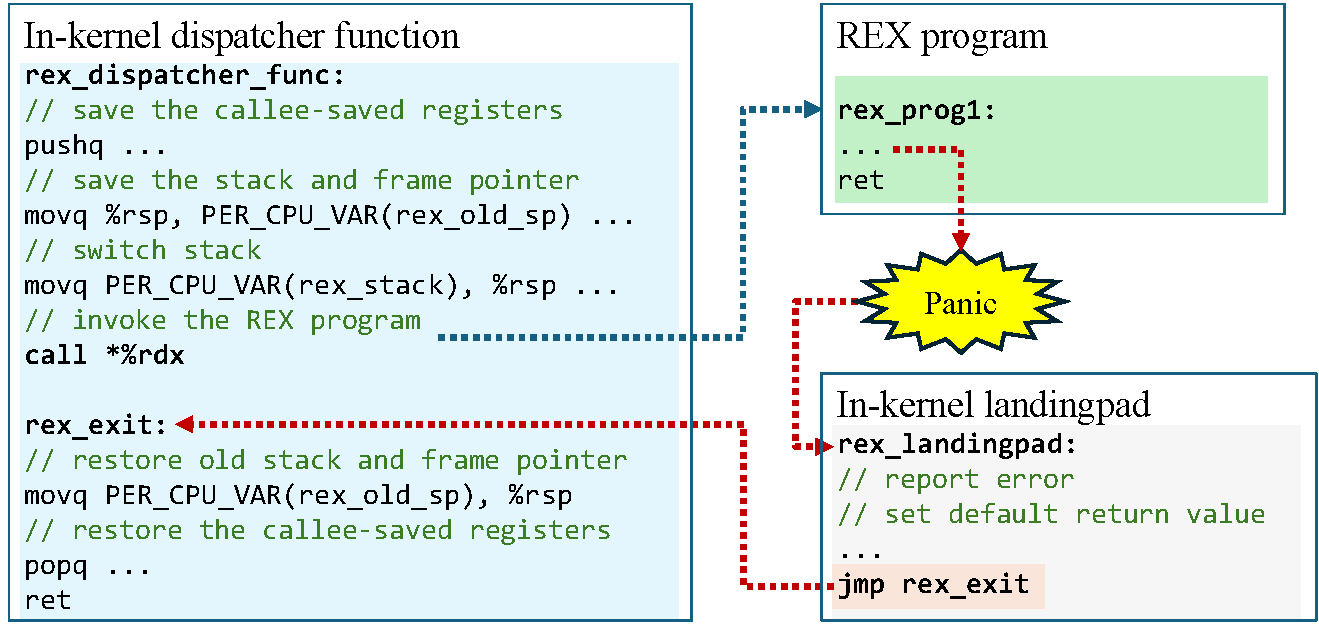
\includegraphics[width=1.0\linewidth]{figs/exception_handling.pdf}
    \centering
    \vspace{-10pt}
    \caption{Exception handling control flow in \projname{}}
    \label{fig:eh-overview}
    \vspace{-10pt}
\end{figure}

Our exception handling framework consists of two components: 1) graceful exit
    upon exceptions that resets the current context and 2) resource cleanup to
    ensure release of kernel resources like reference counts and locks.

\para{Graceful exit:}
To support a graceful exit from an exception, \projname{} implements a small
    runtime (as shown in Figure~\ref{fig:eh-overview}) in the kernel that
    contains a program dispatcher, a panic handler, and a landingpad function.
The dispatcher function takes the same duty of executing the extension program
    as the existing eBPF dispatcher.
It saves the old stack and frame pointer of the current context into per-CPU
    memory before switching to the dedicated program stack
    (\S\ref{principle:stack}) and calling into the program.
If the program exits normally, without triggering an exception, it would
    return to the dispatcher, which switches the stack back.
Under exceptional cases where a Rust panic is triggered, the panic handler will
    release the kernel resources currently allocated by the program, and
    transfer the control flow to the in-kernel landingpad function to print
    debug information related to the exception (e.g., exception message) to the
    kernel ring buffer.
Then, the landingpad function redirects the control flow to a pre-defined label
    in the middle of the dispatcher function, where it restores the old value
    of the stack and frame pointer from the per-CPU storage.
This effectively unwinds the stack and resets the context as if the extension
    program returned successfully.
% We implement the program dispatcher function with panic handling in the kernel
%     in 28 lines of x86 assembly code.

\para{Resource cleanup:}
Light-weight mechanisms can be effective for resource cleanup in \projname{}.
Our insight for resource cleanup is that the extension program can only obtain
    resources by explicitly issuing helper function calls and therefore only
    these resources need to be released.
For these helper function calls, we record the allocated kernel resources
    during execution into a statically defined per-CPU buffer.
Our current implementation can support up to 64
    instances of kernel resources during a single run.
Upon a panic, the panic handler will take the responsibility to correctly
    handle the release of kernel resources, which involves traversing the
    buffer and dropping the recorded resources.
% performing cleanup for each of the recorded resources.

% \jinghao{It seems that nesting should be put somewhere, due to the fact that
% these per-CPU tricks depend on no-nesting.}

We implement the cleanup code as part of the \projname{} kernel crate, as it
    is the core component responsible for coordinating helper function calls
    that obtain kernel resources.
% In this way, the resource cleanup is completely transparent to the extension
%     programs, adding no additional programming burden like the Itanium ABI.
The other reason for implementing cleanup mechanism inside the kernel crate is
    safety, because such code is called upon panic, it must not trigger yet
    another Rust panic and causes panic handling to fail.
Therefore, \projname{} does not execute user-supplied \texttt{drop} handlers
    upon panic, as they are not guarranteed to be safe under panic handling
    context.
%and programs cannot allocate resources without helper function
%    calls.

\subsection{Kernel stack safety}
\label{principle:stack}
One unique safety requirement that kernel extension programs face is the
    usage of kernel stack.
Unlike userspace stacks, which grows on demand with a large maximum size,
    the stack in kernel space is fix-sized (4 pages on x86-64) and limited.
Overflowing the kernel stack may result in memory corruptions or kernel panics.

The eBPF verifier handles stack safety by keeping track of the stack size
    throughout its symbolic execution process.
However, the verification of the stack usage does not always yield the correct
    result -- the verifier has been shown to fail to track stack
    usage across indirect tail calls~\cite{ebpf-stackoverflow}.

Our observation is that the enforcement of stack safety can be easily performed
    at compile time if the extension program does not have indirect or
    recursive calls, and conversely, it is easier to perform such check at
    runtime when the program does employ indirect or recursive calls.
\projname{}, therefore, takes a hybrid approach in ensuring stack safety that
    utilizes static checks for programs without indirect or recursive calls,
    and dynamic, runtime checks for programs make use of such function calls.
For each program being compiled, the \projname{}-specific pass in the compiler
    will check whether it involves indirect or recursive calls.
When the extension program contains only direct, non-recursive function calls,
    its total stack usage can be calculated by traversing its static callgraph
    and sum up the size of each call frame.
If the total stack usage of the program exceeds total amount of stack
    available, the \projname{} compiler pass will generate an error and reject
    the program.

On the other hand, programs with indirect or recursive calls are hard to check
    for stack usage statically, as is the case in the eBPF verifier.
In these cases, \projname{} performs runtime checks to limit the stack usage of
    programs.
The \projname{} compiler pass first ensures each function in the program takes
    less than one page (4K) of stack.
Then, before each function call in the extension program, the pass inserts a
    call to the \texttt{rex\_check\_stack} function.
\texttt{rex\_check\_stack} is provided by the kernel crate and checks the
    current stack depth of the program, if the stack usage exceeds the
    threshold, it will trigger a Rust panic and terminate the
    program safely (\S\ref{principle:eh}).

In order for the \texttt{rex\_check\_stack} function to have more control
    on the stack usage of the program and also support programs with slightly
    large stack usage, \projname{} implements a dedicated kernel stack for the
    extension programs.
The dedicated kernel stacks are allocated per-CPU and virtually mapped during
    kernel boot time with a size of 4 pages.
% the same size as the kernel IRQ and task stacks.
In the dispatcher function (Figure~\ref{fig:eh-overview}), before calling into
    the \projname{} program, the stack and frame pointers of the current
    context are saved.
The dispatcher function then sets the stack and frame pointer registers to the
    top of the dedicated stack and invokes the program.
Upon program exit, the original stack and frame pointers are restored, no
    matter whether a exception is triggered during program execution.

\projname{} defines the stack usage threshold to be 2 pages less than the
    total stack available.
This design choice is based on two considerations.
First, kernel helper functions are not visible at program compile time but they
    also account for stack usage during program execution.
Leaving extra spaces accomodates kernel helper functions and we believe two
    pages of stack is a reasonable limit for kernel helper functions.
Second, since the stack usage of each function in the program is limited to
    1 page of stack, in the worse case, the remaining stack space is at least
    one page when \texttt{rex\_check\_stack} triggers a Rust panic.
This worse case guarantee leaves enough space for the panic handling and stack
    unwinding routines.
Such a dynamic mechanism allows \projname{} to achieve better stack-safety than
    eBPF, which only relies on static verification.

\subsection{Bounded program runtime}
\label{principle:termination}
% A bounded program runtime is important for kernel safety
%   - a potentially long running program can hold the CPU and cause kernel
%     lockups
% eBPF handles this by imposing verification limit (ref S3)
%   (Side note:
%    First, this is really ``bounded runtime'' rather than termination, because
%      a long-running program that eventually terminate is almost equally bad
%    Why would programs ever hit that limit if they are supposed to have an
%    acceptable runtime? Is it because of these two reasons:
%      1. The verifier misses some key information that can reduce the search
%         space drastically, as is the case of unbounded loops?
%      2. If the program is meant to execute that many instructions (current
%         limit is 1M), is it because the current limitation is still too small
%         or is it that the program is badly implemented and actually runs
%         longer? (Also, how long would 1M eBPF instructions run with
%         interpretation and JIT?)
%   )
%   - A program that goes over the limit gets rejected, no matter whether it will
%     actually run long
%   - creates usability issues
%   - previous works has also demonstrated ways of creating long running programs
%     without going over the limit (cite raj-lpc and jinghao-hotos)
%
% Given the ineffectiveness and usability issues associated with the static
%   verification approach, Rex uses a dynamic mechanism that interrupts and
%   terminates programs.
% When a program goes over its time limit, it will be terminated.
% The dynamic termination in Rex limits the runtime of the program through a
%   timer.
% When the timer expires, it issues an IPI to the CPU the program is running.
% The IPI effectively suspends the program and saves its registers to the stack.
% Inside the IPI handler, the timeout handler for Rex is executed, which
%   modifies the instruction pointer stored on the stack to the panic handler
%   of rex programs.
% After returning from the IPI the program will be executing the panic handler
%   to gracefully exit.
%
% Challenge: no termination in helpers/panic handlers
%
% We use a per-CPU flag to solve this

Having a bounded runtime for extension programs is critical for safety of the
    kernel.
A long-running extension program could hold the processor for a long time and
    cause kernel lockups.

eBPF addresses potentially long-running programs by imposing a static limit on
    the number of instructions the verifier would go through.
A program that goes over the instruction limit will be rejected by the
    verifier, no matter whether the program will actually run for a long time.
This techinque creates many false-positives and is one of the main sources of
    the usability issues in eBPF, as discussed in
    \S\ref{motivation:restructure}.
Previous works~\cite{ebpf-termination,untenableVerification} have also
    demonstrated creation of long-running eBPF programs without going over the
    verification limits, further weakening the runtime guarrantee from the
    verifier.

Given the usability issues and ineffectiveness associated with the static
    verification approach, \projname{} employs a dynamic mechanism that
    interrupts and terminates long-running programs at runtime.
% \projname{} supports dynamic program termination through an additional API in the kernel's
% BPF syscall interface.
The dynamic termination in \projname{} limits the runtime of the program
    through a timer.
When the timer expires, it issues an inter-processor interrupt (IPI) to the CPU
    the program is running on.
This IPI effectively suspends the program and pushes its registers onto the
    stack.
Inside the IPI handler, the timeout termination handler of \projname{} is
    executed, which modifies the saved instruction pointer register to the
    panic handler of the program.
After returning from the IPI, the program will be executing the panic handler,
    which cleans up kernel resources allocated by the program and gracefully
    exits the program.
% The termination logic uses the Linux kernel's Inter-Process Interrupt (IPI) mechanism
% to raise an interrupt on the target \projname{} program's CPU.
% Depending on the use-case, the IPI can be triggered by an operator or a timer within the system
% that is configured to notify when the \projname{} exceeds a certain runtime threshold.
% Note that we are assuming the availability of a free CPU for an operator to be able to invoke
% an IPI.
% In uniprocessor machines, where the only CPU will be busy running the extension, the operator
% won't be able to issue termination request and has to rely on installing timers.
% We find this limitation acceptable due to the current cloud infrastructure predominantly being SMP.

% To safely terminate a \projname{} extension, we need to ensure the following :
One challenge involved in terminating a \projname{} program safely is that a
    program should never be terminated while executing the kernel helper
    function or the panic handler, as doing so disrupts internal bookkeeping of
    the kernel (e.g. acquired resources) and safe exception handling process of
    \projname{}.
To address this challenge, \projname{} defers termination when the program is
    running kernel helper functions, and does not attempt to terminate if the
    program is already in the panic handler on the exit path.
% \begin{enumerate}
%     \item A \projname{} program should never be terminated while executing a
%         kernel helper function or the panic handler, as doing so disrupts
%         internal bookkeeping of the kernel (e.g. acquired resources) and safe
%         exception handling process of \projname{}.
%         This is neccesary to ensure kernel objects acquired during a helper call
%         are freed.
%     \item Kernel resources allocated within the extension program cannot be
%         left unreleased and cause resource leaks.
% \end{enumerate}

% The raised interrupt handler first detaches the \projname{} program from its hookpoint to prevent
% further invocation.
% The handler then changes the saved registers(in the interrupt stack) from the \projname{} context
%  to point to the \projname{} panic handler(section \ref{principle:eh}).
% The CPU returns the execution to the panic handler which performs the cleanup of
% any kernel objects that were live at the time of termination.
% To address the case when the target \projname{} program could be inside a helper/panic handler,
% \begin{figure}
%     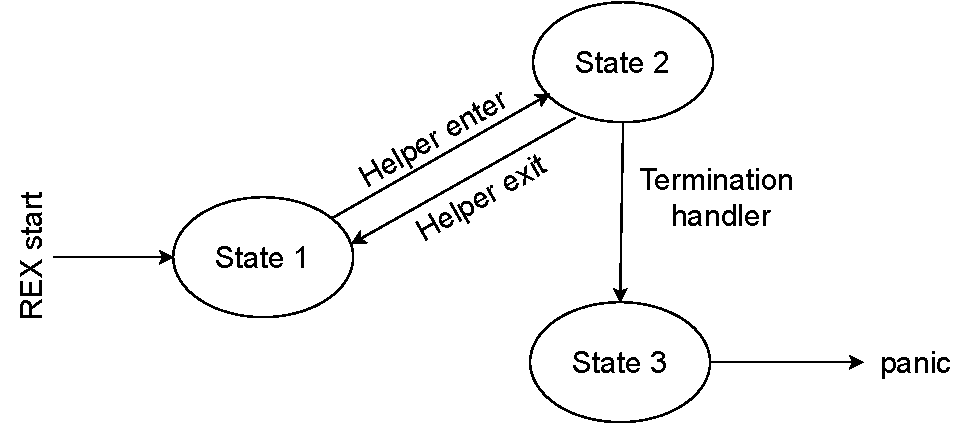
\includegraphics[width=1.0\linewidth]{figs/BPF_termination_state_diagram.pdf}
%     \centering
%     %\vspace{-10pt}
%     \caption{Termination state diagram for \projname{} extensions}
%     \label{fig:rex-termination}
%     %\vspace{-30pt}
% \end{figure}

\projname{} uses a per-CPU tristate flag to keep track the state that the
    extension program is currently in. % (Figure~\ref{fig:rex-termination}).
The states are: 1) executing extension code, 2) executing kernel helpers or
    panic handlers, and 3) termination requested.
Every helper invocation changes the state from state 1) to state 2).
When excuting the timeout termination handler, if the flag is at state 2),
    which indicates the program is in a context that cannot be safely
    terminated, the termination handler modifies it to state 3) without
    setting the instruction pointer.
On a helper function return, the flag is checked and if it is set to state 3),
    the panic handler is called to gracefully exit the program.
% This mechanism is used to defer a panic invocation until the end of a helper execution.
% \jinghao{Shall we have a state diagram?}

\section{Design and Implementation}

\subsection{Design goal}

%\begin{itemize}
%     \item Safety
%         \begin{itemize}
%             \item Same level of safety as eBPF
%             \item Memory safety
%             \item Control-flow soundness
%             \item Resource management
%             \item Program termination
%         \end{itemize}
%     \item Expressiveness
%         \begin{itemize}
%             \item Support more complicated/advanced programs
%             \item Longer programs
%             \item Unbounded loops
%         \end{itemize}
%     \item An important note: we want expressiveness w/o impairing safety (e.g.
%         allow unbounded loop while ensuring termination)
% \end{itemize}

\subsection{Overview}
\begin{itemize}
    \item Brings out the Rust based approach (use Jiyuan's property-oriented
        argument: We want these properties, and Rust happens to provide these)
    \item Infrastructure (Need a figure similar to Fig. 5 from HotOS paper)
\end{itemize}

\subsection{Program load and attachment}
\begin{itemize}
    \item kernel loading code and attachment
    \item relocation fixups for maps and kernel symbols
    \item libiu
\end{itemize}

\subsection{Runtime crate as the programming interface}
\begin{itemize}
    \item overall structure: program type, kernel binding generation, wrapper
        interface around binding.
    \item kernel helper and symbol bindings (dynamic linking scheme)
    \item kconfig-based conditional compilation
\end{itemize}

\para{Kernel symbol resolution}
The \projname{} kernel crate serves as an interface for the extension programs
    to interact with the kernel.
To accomplish this, the crate will need to access kernel symbols.
For example, invoking kernel helper functions requires knowing the kernel
    address of the target helper function symbol.
These kernel symbols includes not only BPF helper functions, but also other
    global and per-CPU variables.

Because \projname{} programs are compiled in userspace, the compiler does not
    have knowledge on any of the required kernel symbols.
One simple solution is to directly passing kernel symbols and their
    corresponding addresses to userspace (e.g. through \texttt{/proc/kallsyms})
However, this is in general considered a dangerous practice as it leaks kernel
    addresses to userspace.
At the same time, this solution is not robust against kernel layout changes
    (e.g. due to kernel rebuild) -- changes of a kernel symbol address requires
    a recompilation of the \projname{} program that uses it.

Our implementation defers the kernel symbol resolution to program load time,
    i.e. when the compiled \projname{} program is sent to the kernel.
At this point, the booted kernel always knows where the symbols are located,
    even after layout changes.
At the same time, the sensitive kernel addresses do not need to be leaked to
    userspace.
\projname{} implements this kernel symbol resolution scheme the same way
    dynamic linking works in userspace.
The compilation process treats all kernel symbols as external and generate
    relocation entries for these undefined symbols.
At load time, the loader library parses the executable, compiles a list of
    kernel sybmols that require resolution with their corresponding entries in
    the global offset table (GOT), and sends the information to the kernel.
The kernel then resolves the address for each symbol via the kallsyms subsystem
    and patches the GOT entries with the resolved addresses and allows programs
    to correctly referencing these kernel symbols.

\para{Kconfig-aware conditional compilation}
% kernel uses config-based conditional compilation
% certain functionalities may not be compiled in
% we also use conditional compilation in kernel crate
% read config from build script and pass to the compilation process
The fact that the Linux kernel employs conditional compilation extensively
    based on kernel configuration values implies that certain functionalities
    used by \projname{} programs may not be compiled in.
An example of this is the ability to override the return value of a function in
    Kprobe programs.
This is only available if the \texttt{CONFIG\_BPF\_KPROBE\_OVERRIDE} is
    enabled.
The \projname{} kernel crate utilizes the conditional compilation counterpart
    in Rust.
The build script of the crate parses the configuration of the kernel for which
    the program is built and send configuration values of interest to the
    compiler.
If a functionality does not have its associated configuration set, its support
    in the kernel crate will not be present, either.

\subsection{Entry code generation}
\begin{itemize}
    \item LLVM pass
\end{itemize}

\subsection{Handle exceptional control flow}
\begin{itemize}
    \item kernel trampoline
\end{itemize}

\subsection{Stack overflow protection}
\begin{itemize}
    \item kernel vmapped, dedicated stack
    \item LLVM instrumentation
\end{itemize}

\subsection{program termination}
\begin{itemize}
    \item Need work
\end{itemize}

\section{Evaluation}

% \begin{itemize}
%     \item Macro-benchmark
%         \begin{itemize}
%             \item BMC
%                 \begin{itemize}
%                     \item Expressiveness: how to evaluate?
%                         \begin{itemize}
%                             \item LOC: we have 33\% reduction
%                             \item 1 rust program vs 7 eBPF programs
%                             \item based on experience?
%                             \item Rust is a safer language
%                         \end{itemize}
%                     \item Performance evaluation
%                         \begin{itemize}
%                             \item Check their paper to see if we can perform
%                                 the same experiment
%                             \item We want a figure similar to Figure 6 in BMC
%                                 (except we don't need to evaluate on different
%                                 CPU configs)
%                             \item x: Vanilla memcached, BMC, Rust
%                             \item y: normalized throughput
%
%                         \end{itemize}
%                 \end{itemize}
%             \item Electrode
%                 \begin{itemize}
%                     \item LOC reduction
%                     \item Performance using their benchmark (similar to figure
%                         5 and 7 in Electrode)
%                     \item Dynamic allocation (ask the authors)
%                 \end{itemize}
%             \item LSM implementation (if we have time / requires handle
%                 nesting)
%             \item XRP
%             \item FUSE in eBPF (from Hubertus)
%         \end{itemize}
%     \item Micro-benchmark
%         \begin{itemize}
%             \item Memory footprint (BPF vs Rust) given we have a larger binary
%                 \begin{itemize}
%                     \item Number of prog in the same translation unit vs memory
%                         usage for program allocation
%                     \item This is because we are always statically linked to
%                         the runtime crate on the translation unit basis
%                     \item E.g. a bpf kern.c with 4 programs vs a rust main.rs
%                         with 4 programs
%                 \end{itemize}
%             \item Small expressiveness examples
%                 \begin{itemize}
%                     \item Loop: strcmp
%                     \item need more
%                 \end{itemize}
%             \item Stack-check overhead
%                 \begin{itemize}
%                     \item Use BMC?
%                     \item Or create some other workload that are function call
%                         intensive (since our instrumentation happens before
%                         each function call)
%                 \end{itemize}
%             \item Cleanup overhead on normal execution path (recording
%                 allocated kernel objects)
%                 \begin{itemize}
%                     \item Similar to Stack-check
%                 \end{itemize}
%             \item Startup overhead due to stack switching
%                 \begin{itemize}
%                     \item A minimal program () to show the upper bound?
%                     \item Plus a real world application (again BMC)?
%                 \end{itemize}
%         \end{itemize}
% \end{itemize}

\subsection{Micro-benchmarks}
\subsubsection{Memory footprint (BPF vs Rust)}
% definition of memory footprint
% eBPF only have JIT code
% Rust have code sections and other sections, e.g. data and GOT sections
We evaluate on how large the in-kernel memory footprint of \projname{} programs
    is comparing to that of eBPF programs.
We define the memory footprint as the number of static memory pages required
    for program execution.
For eBPF, this only includes the JIT-ed native code, since eBPF program does
    not support static data sections.
For \projname{} this includes all load segments from the compiled ELF
    executable, which consists not only the text sections, but also the data
    sections for static variables (e.g., program objects and maps objects) as
    well as the sections that implement support for position-independent code
    (e.g., GOT sections).

In this experiment, we compare the number of memeory pages required for both
    \projname{} programs and their equivalent eBPF programs.
We select 3 simple eBPF programs from the sample eBPF programs shipped with the
    kernel -- the trace point program \texttt{syscall\_tp}, the kprobe program
    \texttt{tracex5} and the perf event program \texttt{trace\_event}.
We also include the BMC program (\S~\ref{eval:macro}) in the experiment because
    it represents an example of a complicated eBPF program.
For all the programs, we implement a \projname{} version with the same
    overall logic.

\begin{itemize}
    \item need a figure: bar graph showing the memory footprint of bpf and
        \projname{} programs on our sample programs
    \item sample programs: \texttt{syscall\_tp}, \texttt{tracex5},
        \texttt{trace\_event}, and BMC.
    \item y: total number of pages allocated for the loaded object (JIT-ed code
        for BPF, loaded and mapped pages for Rust)
\end{itemize}

\jinghao{Discussion on the result really needs the result, I am not sure which
one will have a smaller memory footprint.}

\subsubsection{Startup overhead due to stack switching}
\begin{table}[t]
    \small
    \centering
    \begin{tabular}{cc}%{|p{6cm}|p{1cm}|}
        \toprule
        \textbf{Extension} & \textbf{Runtime of empty program (ns)} \\
        \midrule
        eBPF & 43.5 $\pm$ 4.79 \\
        \projname{} & 44.1 $\pm$ 4.93 \\
        \bottomrule
    \end{tabular}
    \caption{Runtime of an empty program for eBPF and \projname{}}
    \vspace{-10pt}
    \label{tab:startup-overhead}
\end{table}

\projname{}'s usage of a dedicated stack for execution and the implementation
    of exception handling support may incur additional overhead during program
    startup and shutdown.
This design requires saving of the stack and frame pointer and replacing them
    with the top address of the dedicated stack before starting the program,
    and restoring the saved stack and frame pointer after the program exits.
The manipulation of the stack pointers adds to six more memory instructions to
    the dispatcher function of the \projname{} programs.
In this experiment we measure the overhead of these stack pointer operations.
We implement an empty kprobe extension program -- both in eBPF and in
    \projname{} -- and measure their wall runtime including the program
    dispatcher function.
The result is shown in Figure~\ref{tab:startup-overhead}.
On average, the difference of runtime of invoking an empty \projname{} and eBPF
    program is less than 1ns.
This shows the additional stack manipulations needed by \projname{} does not
    contributed to non-negligible overhead.

\subsubsection{Verifier/JIT-based optimization}
\label{eval:inline}

% The raw data and script used to make the graph (plot2.py)
% is in the map-test directory under testing/analysis/
% With the three files: ['elapsed_times_5.15.csv',
%    'elapsed_times_5.15_non_inlined.csv', 'elapsed_times3-rust.csv']
% Corresponding to the bars
% Link to it: https://github.com/rosalab/map-test/tree/main/testing/analysis

\begin{figure}
    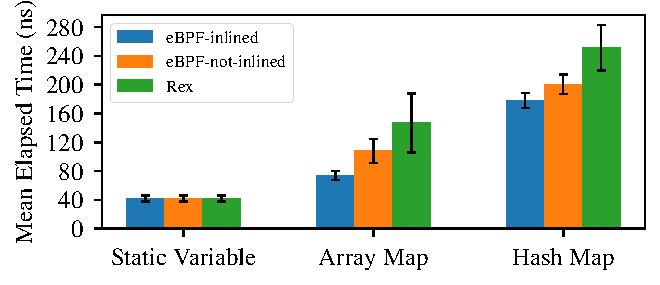
\includegraphics[width=1.0\linewidth]{figs/inline.pdf}
    \centering
    \vspace{-25pt}
    \caption{Runtime of map lookups on various setups}
    \label{fig:eval-inline}
    \vspace{-10pt}
\end{figure}

% \begin{itemize}
%     \item inline v.s. out-of-line map helpers
%         \begin{itemize}
%             \item table showing runtime of a map lookup operation in a eBPF and
%                 a Rust program
%             \item the kernel will automatically inline lookup in BPF
%             \item Rust version will not get inlined
%             \item measurement can be in ns for now, but better if it could be
%                 in cycles
%             \item maps to test: array, hash (htab-lru, xsk-map?)
%         \end{itemize}
% \end{itemize}

We evaluate the impact of missed opportunities due to the elimination of the
    eBPF verifier in \projname{}.
Specifically, we look into the optimization of eBPF map lookups.
For eBPF programs, the verifier can inline the \texttt{bpf\_map\_lookup\_elem}
    helper function by replacing the call into equivalent eBPF instructions.
This optimization can avoid two function calls and two pointer dereferences for
    map types that support lookup inlining.
However, in \projname{}, inlining is not performed due to the absence of the
    eBPF verifier as well as kernel internal information (e.g. map addresses).

In this experiment we measure the runtime of eBPF map lookups under three
    settings, eBPF with inlining, eBPF without inlining, and \projname{}.
Our test program for both eBPF and \projname{} is a tracepoint program that
    uses the \texttt{bpf\_ktime\_get\_ns} helper to measure the runtime of
    a \texttt{bpf\_map\_lookup\_elem} call.
The \texttt{bpf\_map\_lookup\_elem} invocation is by defualt inlined by the
    eBPF verifier when possible.
The setup of eBPF without inlining is achieved by removing the inlining logic
    from the eBPF verifier.
We selected two commonly-used eBPF map types for this experiment: array maps
    and hash maps.
Both of them support lookup inlining.

% Figure~\ref{fig:eval-inline}
% shows the performance of inlining and non-inlining on a vanilla
% v5.15 kernel as well as the \projname{} implementation.
Figure~\ref{fig:eval-inline} shows the performance of map lookups under the
    three different setups on different maps.
% The vanilla non-inlined
% kernel is achieved by commenting out the lines in the kernel verifier.c file that
% automatically inlines the bpf\_map\_lookup\_elem method.
For both array maps and hash maps, the
    runtime of map lookup can be reduced by 20-30 ns compared to eBPF without
    inlining.
% In the graph,
% the performance impact of inlining the method is 20-30 nanoseconds.
% The additional slowdown of 30-40 nanoseconds seen in the rust implementation
% can be explained by the wrapping performed around the bpf\_map\_lookup\_elem method.
An additional slowdown of 30-40 nanoseconds is present for map lookups in
    \projname{}.
This is because of the wrapping code around the kernel
    \texttt{bpf\_map\_lookup\_elem} that allows \projname{} programs to invoke
    it using safe Rust objects.

% Egor: Not sure if I should go into more technical details about whats going on
% in the wrapping

% Using libbpf (and libiu in the case of \projname{}) the sample \projname{} or c bpf
% program is loaded and attached to a tracepoint which is then called by the trigger.
% In the instance of the inlined and non-inlined tests this tracepoint is getcwd, and
% in the instance of the rust tests that tracepoint used is sys\_enter\_dup. The
% triggers consist of a one-line c program that calls the appropriate function such as getcwd().
% The bpf program creates the corresponding map and measures the time
% it takes to execute a single map\_lookup\_elem. This time is measured with
% bpf\_ktime\_get\_ns() and then printed with bpf\_printk() and recorded.
% \milo{Maybe we should talk about why we chose these specific maps. i.e. that array and hash maps are the main ones that support the inlining?}

\subsubsection{Stack-check overhead}
\begin{itemize}
    \item table showing runtime of two programs using small recursion
    \item eBPF: use tail calls for recursion
    \item Rust: just a recursive function
    \item The recursion count should not be statically known to prevent llvm
        from optimizing out the recursion
\end{itemize}

We then evaluate how much overhead the runtime stack check have on the
    performance of \projname{} programs.
The stack instrumentation is added before each
    function call in the \projname{} program if the program contains indirect
    or recursive function calls that prevents the compiler from calculating the
    stack usage statically.
In this experiment we implement recursive factorial computation program in both
    eBPF and \projname{}.
Since eBPF does not natively support recursive functions, we use eBPF tail
    calls to invoke the same program.
At same time, because recursive factorial computation can always be tail-call
    optimized in Rust, this comparison should be able to precisely highlight
    the performance implication of the runtime stack instrumentation.
\jinghao{TODO: discuss results.}

\subsubsection{Cleanup overhead on normal execution path}
\begin{table}[t]
    \small
    \centering
    \begin{tabular}{cc}%{|p{6cm}|p{1cm}|}
        \toprule
        \textbf{Extension} & \textbf{Runtime of acquiring \& release a lock (ns)} \\
        \midrule
        eBPF & 256.8 $\pm$ 142.4 \\
        \projname{} & 254.5 $\pm$ 192.3 \\
        \bottomrule
    \end{tabular}
    \caption{Runtime of spinlock acquire and release for eBPF and \projname{}}
    \vspace{-10pt}
    \label{tab:cleanup-overhead}
\end{table}

The cleanup mechanism employed by \projname{} requires recording the allocated
    resource at runtime, which comparing to eBPF or Itanium C++ ABI, adds extra
    runtime overhead.
We therefore evaluate the runtime overhead from \projname{}'s cleanup
    mechanism.
For this miscrobenchmark, we choose to use a program that acquires and then
    immediately releases a BPF spinlock.
Since the acquired spinlock is a resource that needs to be released upon Rust
    panics, \projname{}'s cleanup mechanism needs to record it in its per-CPU
    buffer.
The program is implemented both in eBPF and \projname{} and the time used to
    acquire and release the spinlocks are measured.
As shown in Table~\ref{tab:cleanup-overhead}, the runtime difference between
    eBPF and \projname{} is less than 2ns with \projname{} being the faster
    one, implying the overhead of \projname{}'s cleanup mechanism is
    negligible.

\subsection{Macro-benchmarks}
\label{eval:macro}
We now demonstrate that \projname{} can be used to implement complicated,
    real-world kernel extension use cases with enhanced usability but without
%    losing much performance by implementing BMC and Electrode in \projname{}.
    losing much performance by implementing the BPF Memcached Cache (BMC) in
    \projname{}.

% \subsubsection{\projname{}-based BMC}
% \jinghao{TODO: Preamable}
% BMC implements in-kernel memcached cache -- how it works
% Compilcated program, original paper splits into 7 programs and uses tail calls
%

BMC~\cite{BMC} is an in-kernel cache for Memcached based on eBPF.
It stores recently queried key-value pairs in an eBPF map to accelerate the
    processing of GET requests to the Memcached server.
If a GET is hit in the cache, the queried value can be sent in a reply without
    going through the expensive network stack in the Linux kernel.
The map that servers as the cache is managed by eBPF programs, which implements
    the lookup and update logics.

On the aspect of implementation, BMC is a much more complicated program
    comparing to other common eBPF use cases.
In order to pass the verifier, the implementation has to be splitted into seven
    eBPF programs that tail-calls into each other to reduce verification
    complexity.
Similar problem also presents when processing the incoming packet data, where
    the authors had to bound data size to reduce verification complexity for
    loops.

We re-implement BMC in \projname{} (\projname{}-BMC) to demonstrate the
    enhanced usability without losing performance.
The resulting program is not a direct translation from the original eBPF
    version in C, rather, we implement the same high-level logic but with
    slight deviations from BMC where the enhanced usability and expressiveness
    of Rust allows a simpler implementation.

% The BMC has many places where for loops are nested into different ifs.
% And, due to the limitations of C, many operations do not have built-in functions
%     that can be used directly.


In the initial design of \projname{}-BMC, the underlying assumption was that
    we should follow the logic of BMC.
But the cache invalidation function in BMC employs
    for loops with cumbersome condition checks, and is further
    complicated by the nesting of multiple if statements.
The complexity is exacerbated by introducing two additional variables to track
    special states.
\jinghao{What states? It does not need to be too detailed.}
Such complex conditional judgments will significantly undermine the readability
    of the BMC code, and it may lead to ambiguities in some places regarding
    the intended functionality.
\jinghao{Can we make the claim that this complexity is for passing the
    verifier?}
% During implementation of function \texttt{bmc\_invalidate\_cache},
%     we assume that each pcket

% However, subsequent testing revealed the possibility of multiple set commands
%     within a single packet.

% This discovery highlighted the obscurity and susceptibility to errors inherent
%     in the original code structure, primarily due to the complex judgment
%     conditions buried within nested if statements.

To address these challenges, \projname{}-BMC utilizes the lazy-evaluated
    \texttt{filter\_map} function from Rust iterators.
\jinghao{What are these challenges -- are we still in the context of cache
    invalidation? By the way, can we abstract this out to all ``loops'' in BMC?
At the same time, we probably need to explain what \texttt{filter\_map} does.}
This approach facilitates the creation of an iterator, which is instrumental in identifying
    the quantity of SET commands present in the current packet payload.
Further enhancing the readability, Rust's syntactic sugar is employed for
    iterating over the identified memcached SET commands, streamlining the process.
The complexity of the original code, characterized by four levels of nesting,
    is significantly reduced by converting a for-loop with intricate conditions
    into a lambda function.
\jinghao{lambda function -> a clean chain of higher-order functions with
    lambda function?}
This conversion is achieved through the utilization of \texttt{take\_while}
    combined with generated iterator, thus dividing the code into three distinct
    sequential parts and markedly improving its expressiveness.
\jinghao{Also should explain what \texttt{take\_while} does.}

\jinghao{Now it feels like we should make part larger, i.e., include code
    examples and show how Rust helps with that.
We can then move this part into the new qualitative evaluation.}

%\para{Experiment setup}
Our evaluation setup consists two machines, with one
    acting as the server and the other one acting as the client.
The server machine runs the \projname{} custom kernel based on Linux v5.15.0 on
    an AMD EPYC 7551P 32-Core processor with 112 GB memory.
SMT and Turbo are turned off for the experiments.
The client machine runs a vanilla v6.8.0 Linux kernel on AMD Ryzen 9 7900X
    processor with 128 GB memory.
Both machines are equiped with Mellanox ConnectX-3 Pro 40GbE NICs and are
    connected back-to-back using a single port.

% Key: 16 bytes, value: 32 bytes
% 50 million with Zipf 0.99
% 10 GB memcached, 2.5 GB BMC
% Preload all keys
% GET:SET 30:1

We use the following workload to evaluate our \projname{}-BMC together with the
    original eBPF-BMC.
Our dictionary contains 50 million Memcached keys following a Zipf
    distribution with 0.99 skewness.
All keys are 16 bytes in size and are paired with 32-byte values in the
    experiments.
The storage sizes of the Memcached and BMC are set to 10 GB and 2.5 GB,
    respectively.
According to the calculation in the original work, all items
    can be stored in Memcached itself but only 6.3 million of them can fit in
    BMC.
Before experiments, the Memcached server is pre-loaded with all keys by
    sending TCP SET requests for each key in the dictionary from the client.
The client then sends requests to the server with a 30:1 ratio betweren UDP GET and
    TCP SET requests and measures the throughput.

We evaluate the throughput of three setups: MemcachedSR (from BMC),
    MemcachedSR+BMC, and MemcachedSR+\projname{}-BMC.
The original open-sourced BMC code targets Linux kernel version 5.3.0 and we
    port it to the v5.15.0 \projname{} kernel for the evaluation.
For each setup, we vary the number of processor cores and the number of threads
    used by the Memcached server and pin each thread onto each core.
We also adjust the CPU affinity of IRQs associated with the NIC such that the
    network interrupts are processed on the same set of cores the Memcached
    server executes on.

\begin{figure}
    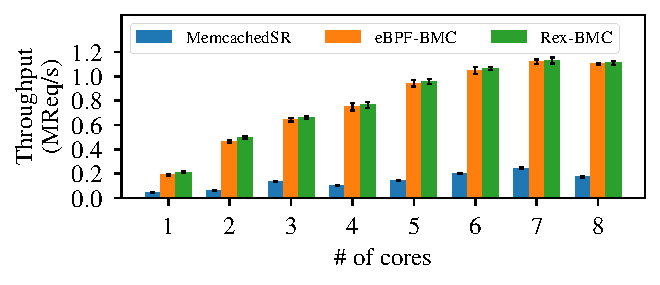
\includegraphics[width=1.0\linewidth]{figs/bmc.pdf}
    \centering
    \vspace{-25pt}
    \caption{Throughput of BMC on MemcachedSR, eBPF-BMC, and \projname{}-BMC
        under different number of CPUs/threads.
    }
    \label{fig:eval-bmc}
    \vspace{-10pt}
\end{figure}

Figure~\ref{fig:eval-bmc} shows the throughput of the three setups under
    different numbers of CPUs and threads.
MemcachedSR processes all requires in userspace and thus its throughput suffers
    from the overhead of the kernel network stack, achieving only 45K requests
    per second under a single thread and 175K requests per second under 8
    cores.
On the other hand, both eBPF-based and \projname{}-based BMC are able to
    achieve a much higher throughput because they can process a large
    fraction of requests at NIC level and without the need of going through
    the expensive kernel network stack.
With 8 CPU cores and threads, eBPF-BMC and \projname{}-BMC achieve a thoughput
    of 1.106M and 1.111M, and a performance benefit of 6.3x and 6.4x,
    respectively.
It is also clear that \projname{} is able achieve a better usability while
    keeping the same level of performance and safety guarrantee comparing to
    eBPF,  as the throughput of \projname{}-BMC is comparable to that of
    eBPF-BMC under all CPU/thread setups.

\section{Discussion}
\begin{itemize}
    \item Unsafe code in rt crate
    \item Verified Rust extension using Verus
    \item Dynamic allocation (if we end up not doing it)
    \item Cross-Language Attacks from NDSS 2022
    \item Rust memory ordering in kernel (\url{https://lwn.net/SubscriberLink/967049/66bfb6f365d164aa/})
\end{itemize}
\section{Related Work}
\subsection{Rust-based system}
\begin{itemize}
    \item Theseus
    \item Redleaf
    \item Evolving Operating Systems Towards Secure Kernel-Driver Interfaces
    \item Michael Swift works
    \item Leveraging Rust for Lightweight OS Correctness
    \item Cross-Language Attacks from NDSS 2022
\end{itemize}

%\subsection{Other eBPF safety}
\subsection{Unprivileged eBPF through Extra Safety}
Other work has attempted to add additional safety to eBPF programs largely
    to support unprivileged eBPF.
MOAT~\cite{lu2023moat} uses hardware based Intel Memory Protection Keys
    to isolate eBPF programs from the kernel.
This would prevent attackers from using eBPF.
Another system SandBPF~\cite{sandbpf} uses software fault isolation to dynamically
    sandbox eBPF programs.

\subsection{Other OS extension}
A large body of work exists around the theme of creating extensible operating systems.
Systems such as SPIN \cite{spin} utilize the type safety of Modula-3 to produce safe extensions that dynamically link into the kernel.
VINO \cite{vino} uses software fault isolation techniques and interposition to allow for kernel functions to be replaced, or event-based extensions to be implemented.
Similarly, SLIC \cite{slic} uses interposition as a mechanism to allow trusted extensions to be run with only minimal operating system changes.

\section{Experience}
% \begin{itemize}
%     \item XDP/Sched-cls kernel crate problem: commit a70dffa0
%     \item Triggering Rust exception when implementing BMC, but kernel is still
%         alive.
% \end{itemize}
\para{Rex Panic Handler}
During the debugging of cache miss rate issues in BMC, we observed that the
\texttt{bmc\_invalidate\_cache} function in the Rex version failed to deliver expected
    results via the statistical records.
This discrepancy indicated a potential flaw in that function's implementation
    or its interaction with the cache map.

    Then we attempted to utilize \texttt{bpf\_printk (Rex version)} for diagnostic, but
    the logging results was absence from the tracing files,
    and the \projname{}-BMC has a significant degradation in benchmark performance.
Reverting these changes restored the original performance levels and logging capabilities.

Afterwards, examination of the kernel logs showed an shocking number of kernel error messages.
With further investigation of these log along with the code, an out-of-bounds access error
emerged from the \texttt{bmc\_invalidate\_cache} function.
This mistake was the cause of kernel panics observed during benchmark.

Remarkably, even with the numerous kernel panics, the overall system stability
    and performance were not conspicuously impacted.
We have run several benchmarks in this kernel which already has a lot of Rex panic
    and this kernel continued to function well.
This resilience highlights an robustness in the unwind implementation of Rex.


\section{Conclusion}
This paper identifies the fundamental \gap{} within the current Linux eBPF
    infrastructure that is the source of its poor usability.
We make the observation that by using a safe language for kernel extensions and
    remove the extra verification layer, both the desired usability and safety can be
    achieved.
We demonstrate this by presenting \projname{}, a Rust-based kernel extension
    framework for the Linux kernel that leverages language-based safety from
    Rust without a separate verfier.
We show that \projname{} is able to solve existing usability issues
    associated with the eBPF verifier without performance costs, facilitating
    safe and easy-to-write kernel extensions.
%%
%% The next two lines define the bibliography style to be used, and
%% the bibliography file.
\bibliographystyle{acm}
\bibliography{ref}

% \appendix
\appendix
\section{Appendix}
% \label{sec:impl}

\jinghao{\S\ref{sec:impl}: How to make it work}

% \subsection{Design goal}

%\begin{itemize}
%     \item Safety
%         \begin{itemize}
%             \item Same level of safety as eBPF
%             \item Memory safety
%             \item Control-flow soundness
%             \item Resource management
%             \item Program termination
%         \end{itemize}
%     \item Expressiveness
%         \begin{itemize}
%             \item Support more complicated/advanced programs
%             \item Longer programs
%             \item Unbounded loops
%         \end{itemize}
%     \item An important note: we want expressiveness w/o impairing safety (e.g.
%         allow unbounded loop while ensuring termination)
% \end{itemize}

% \subsection{Overview}
% \begin{itemize}
%     \item Brings out the Rust based approach (use Jiyuan's property-oriented
%         argument: We want these properties, and Rust happens to provide these)
%     \item Infrastructure (Need a figure similar to Fig. 5 from HotOS paper)
% \end{itemize}

We now discuss the high-level mechanisms that we use to build various features in
    \projname{} and make it a practical kernel extension framework.
These include the following:
\begin{itemize}
    \item How the \projname{} kernel crate bridges programs and the kernel.
    \item How \projname{} programs are loaded and attached.
    \item How eBPF maps are supported in \projname{}.
    \item How is the entry of \projname{} implemented that allows kernel to
        execute them directly.
\end{itemize}

\subsection{\projname{} kernel crate}
% \begin{itemize}
%     \item overall structure: program type, kernel binding generation, wrapper
%         interface around binding.
%     \item context conversion
%     \item kernel helper and symbol bindings (dynamic linking scheme)
%     \item kconfig-based conditional compilation
%     \item Map support
% \end{itemize}

The \projname{} kernel crate is responsible for supporting interactions between
    kernel and \projname{} programs and contains interfaces facing both sides.
% It contains support for different program types with
%     interfaces facing the kernel and the \projname{} program.
\projname{} support the same set of program types as eBPF.
Each program type is defined as a Rust struct and with allowed helpers defined
    as its methods.
This effectively implements access control on helper functions with respect to
    program types (e.g., a tracing program should not modify socket buffers
    through networking helper functions), which is also present in eBPF.
The user defines a program object of one of the program struct types and
    assoociates it with a Rust function as the extension program.
The extension function takes in the associated program object and the
    program-type-specific context from the kernel as arguments
    (\S\ref{impl:ctx-converison}).
Inside the extension, developers can use Rust kernel bindings generated by the
    crate to access kernel structures (\S\ref{impl:crate:binding}).
At the same time, helper functions allowed for the program type can be
    invoked through the program object, which are backed by eBPF kernel helpers.
    (\S\ref{impl:crate:symbol-resolv}).

% The crate also has support for maps (\S\ref{impl:map}) and other
%     miscellaneous utilities for the ease of programming (e.g. wrapping return
%     code in \texttt{Result} to support monadic operations in Rust).

\subsubsection{Supplying program context}
\label{impl:ctx-converison}
% Like eBPF, \projname{}
Extension programs take in a kernel-provided ``context'' as input argument.
The context is a pointer to a struct that contains information the program may
    need.
The current eBPF keeps a pair of context struct definitions for certain program
    types, where one of them is exposed to extension programs and the other one
    is the internal data structure in the kernel.
The extension-facing definition is generally a subset of the associated kernel
    internal definition.
This is done for the reason of keeping a stable interface and hidding unneeded
    kernel data from the extension programs.
When a eBPF program is loaded into the kernel, the verifier rewrites accesses
    into the corresponding field in the kernel context
    through the verifier hook specific to the program type.
Rewriting the access also avoids the need for copying data and contructing an
    extension-facing context.

% In \projname{}, the Rust compiler takes the place of the eBPF verifier and as
%     a result there is no way to rewrite the access to the context the same
%     way eBPF does.
In \projname{} the removal of the verifier means it cannot rewrite the access
    to the context the same way eBPF does.
Instead, \projname{} take the advantage of the expressive Rust language
    features.
In particular, \projname{} exports to the extension programs a struct that just
    wraps around the pointer to kernel context.
It implements accesses to the needed fields in the kernel context as safe Rust
    methods of this struct, which accesses the kernel struct internally via
    generated bindings (\S\ref{impl:crate:binding}).
% Doing so effectively re-route accesses to the kernel struct.
At the same time, it also allows controlled access to the kernel context and
    prevents unwanted writes to the context, which may corrupt kernel data
    accidentally.

\subsubsection{Creating Rust bindings of kernel structs}
\label{impl:crate:binding}
Extension programs rely heavily on the kernel data structure definitions.
A tracing program may want to obtain information from the kernel
    \texttt{task\_struct}, while a networking program needs to know the layout
    of protocol headers.
In eBPF, the need can be easily full-filled by including the corresponding
    kernel header files, as most of the time the program is implemented in C
    and compiled to eBPF bytecode.

The problem becomes more involved in \projname{}, as it uses Rust as the
    programming language, which cannot directly work with kernel C headers.
% As a solution, \projname{} creates Rust bindings for the needed kernel
%     definitions.
As a solution, \projname{} uses Rust-bindgen~\cite{bindgen} to create Rust
    bindings for kernel structure definitions and constants from kernel header
    files.
\projname{} integrates the binding generation into program compilation so that
    the bindings are automatically generated for the target kernel during
    build.
The generated Rust binding forms part of the kernel crate and can be imported
    into \projname{} programs like other contents of the kernel crate.

\subsubsection{Supporting kernel helper functions}
\label{impl:crate:symbol-resolv}
Kernel extensions utilizes kernel helper functions for perform more advanced
    operations.
eBPF uses kernel helpers as both a way to interact with the kernel and to
    complement its limitation on expressiveness.
\projname{}, on the other hand, only uses helpers for kernel interaction, since
    Rust is expressive enough that it does not need additional helper functions.

\projname{} uses the existing eBPF helper interface and implements on top of
    it a Rust wrapping layer.
This wrapping layer serves to hide the unsafe kernel C helper interface and
    provides a new interface that \projname{} programs can safely use.
The implementation of eBPF map lookup helper is shown in
    Figure~\ref{fig:map-helper}.
On L30, the kernel helper function returns a pointer to the map value
    (\texttt{*mut V}), the \projname{} wrapping layer converts the pointer
    into a Rust option type~\cite{rust-option} (\texttt{Option<\&mut V>}) on
    L33-L37, which allows \projname{} programs to access the object through a
    safe Rust reference without worrying about deferencing a null pointer.

\begin{figure}[t]
    \lstinputlisting[language=Rust]{./snippets/s5-map.rs}
    \vspace{-10pt}
    \caption{Implementation of eBPF map support in \projname{}}
    \vspace{-10pt}
    \label{fig:map-helper}
\end{figure}

In eBPF, most of the helper calls are direct function calls, however, a few of
    them are further optimized during verification and JITing.
Helper functions in \projname{} do not have the same load time optimization,
    and at the same time the kernel crate wraps the unsafe kernel helpers with
    a safe Rust interface, which could incur further overhead.
We further evaluate the impact in \S\ref{eval:inline}.

% For required kernel symbols (e.g., kernel helper functions), the kernel crate
%     creates a stub declaration for each symbol without using Rust-bindgen.
% This is because certain kernel symbols -- especially all eBPF helper
%     functions --  do not have a declaration in kernel header files.
% The actual definition of the kernel symbols will be resolved when the program
%     is loaded into the kernel (\S\ref{impl:crate:symbol-resolv}).

% The \projname{} kernel crate serves as an interface for the extension programs
%     to interact with the kernel.
% To accomplish this, the crate will need to access kernel symbols.
To reuse the existing kernel helper interface, the crate will need to access
    kernel symbols.
At the same time, the crate itself may also need to access certain kernel
    symbols for internal house keeping operations (e.g. resource cleanups as in
    \S\ref{principle:eh})
% For example, invoking kernel helper functions requires knowing the kernel
%     address of the target helper function symbol.
% These kernel symbols includes not only BPF helper functions, but also other
%     global and per-CPU variables.
Because \projname{} programs are compiled in userspace, the compiler does not
    have any knowledge on the required kernel symbols.
% One simple solution is to directly passing kernel symbols and their
%     corresponding addresses to userspace (e.g. through \texttt{/proc/kallsyms})
% However, this is in general considered a dangerous practice as it leaks kernel
%     addresses to userspace.
% At the same time, this solution is not robust against kernel layout changes
%     (e.g. due to kernel rebuild) -- changes of a kernel symbol address requires
%     a recompilation of the \projname{} program that uses it.

\projname{} therefore defers the kernel symbol resolution to program load time,
%     i.e., when the compiled \projname{} program is sent to the kernel.
    the same way dynamic linking works in userspace.
At this point, the booted kernel always knows where the symbols are located.
%     even after layout changes.
% At the same time, the sensitive kernel addresses do not need to be leaked to
%     userspace.
% \projname{} implements this kernel symbol resolution scheme the same way
%     dynamic linking works in userspace.
The \projname{} kernel crate merely creates stub declarations for the required
    kernel symbols.
During compilation, the compiler treats all kernel symbols as external and
    generate relocation entries for the undefined symbols.
At load time, the loader library (\S\ref{impl:load}) parses the executable,
    compiles a list of kernel sybmols that require resolution with their
    corresponding entries in the global offset table (GOT), and sends the
    information to the kernel.
The kernel then resolves the address for each symbol via the kallsyms subsystem
    and patches the GOT entries with the resolved addresses.
This allows programs to access kernel symbols without the need to disable
    kernel address space layout randomization (KASLR).
% and allows programs to correctly referencing these kernel symbols.

\subsubsection{Kconfig-aware conditional compilation}
% kernel uses config-based conditional compilation
% certain functionalities may not be compiled in
% we also use conditional compilation in kernel crate
% read config from build script and pass to the compilation process
The fact that the Linux kernel employs conditional compilation extensively
    based on kernel configuration values implies that certain functionalities
    used by \projname{} programs may not be compiled in.
An example of this is the ability to override the return value of a function in
    Kprobe programs.
This is only available if the \texttt{CONFIG\_BPF\_KPROBE\_OVERRIDE} is
    enabled, which is checked by the verfier in current eBPF.
The \projname{} kernel crate utilizes the conditional compilation counterpart
    in Rust.
The build script~\cite{rust-build-script} of the crate parses the configuration
    of the target kernel and send configuration values of interest to the
    compiler.
The compiler the conditionally compiles the code guarded by the configurations.
If a functionality does not have its associated configuration set, its support
    in the kernel crate will not be present, either.

\subsection{Program load and attachment}
\label{impl:load}
% \begin{itemize}
%     \item kernel loading code and attachment (w/ base program)
%     \item relocation fixups for maps and kernel symbols
%     \item libiu
% \end{itemize}
% Difference between eBPF and Rust programs
% - native code vs. byte code + JIT
% - no verifier to fixup relocations for maps and kernel symbols (e.g helpers)
% Implement kernel side loading logic
% - allocate page and map all LOAD segments in the ELF executable
% - fix all relocations for maps and kernel symbols
% - use the same eBPF insfrastructure
% problem where programs within the same executable share code
% - multiple programs calling the same function
% - one copy per program is ineffcient on memory
% - solution: first load the ELF executable, then associate individual programs
%   with extension entry functions in the code
There are two major differences between eBPF and \projname{} that poses unique
    challenges to the loading of \projname{} programs in the kernel.
Firstly, \projname{} is loaded as native code after compilation, of which the
    kernel does not have control on the layout.
This means the kernel need to parse and handle different sections in the
    program differently.
In contrast, eBPF is loaded as eBPF bytecode and contains only executable code.
The kernel has complete control over the generated native through the kernel
    eBPF JIT infrastructure.
Secondly, \projname{} does not have the in-kernel verifier, which is used in
    eBPF to fixup the kernel objects the program references (e.g., maps and
    helpers).
Therefore, the loading logic also needs to perform fixups needed for
    \projname{} on relocations.

The loading of a \projname{} program can be divided into two phases, with the
    first one happening in userspace and the other in kernel space.
The first phase is responsible for parsing the ELF executable into a format the
    kernel can understand as well as performing prerequisite operations (e.g.,
    creation of eBPF maps).
In \projname{} this is done by its userspace loader library \texttt{librex}.
Similar to how \texttt{libbpf} operates on eBPF programs, \texttt{librex}
    provides routines that parses the eBPF maps, kernel symbol relocations,
    and programs from the \projname{} ELF executable.
Once the sections are parsed, it creates the eBPF maps and update the
    corresponding map entries in the ELF (\S\ref{impl:map}), and then load
    the program by sending the ELF binary as well as the map and relocation
    information.
Parsing the ELF sections in usrspace avoids complexity of the loading logic in
    the kernel.

For the second phase, we extend the \texttt{bpf} system call to support loading
    of \projname{} programs.
The system call sends the compiled ELF executable as well as the associated
    relocation information into the kernel.
The kernel first parses the ELF executable and locate all the \texttt{LOAD}
    segments in the executable.
It then allocate new pages and maps the \texttt{LOAD} segments into the
    kernel address space based on the size and permissions of the segments.
With the associated relocation information, the kernel updates the kernel
    symbol relocation entries (\S\ref{impl:crate:symbol-resolv}) and eBPF maps
    (\S\ref{impl:map}) with the corresponding absolute address in the kernel.
% The relocations that need fixup are kernel symbols referenced by the
%     \projname{} program (\S\ref{impl:crate:symbol-resolv}) and eBPF maps
%     (\S\ref{impl:map}).
At this point, the program is considered ``loaded''.
The kernel then wrap the program into a \texttt{bpf\_prog} struct as if it is a
    JIT-ed program -- reusing the existing eBPF infrastructure for program
    management greatly reduces engineering efforts and facilitates easy
    integration with existing eBPF hook points.

Kernel extensions often involves use cases where multiple programs are defined
    together and share common code in the same executable.
% One of the problem \projname{} faces is to deal with multiple programs within
%     the same ELF executable.
% Such programs may share common code in the same executable.
eBPF loads each of the program independently and deplicates the shared code. \jinghao{need check}
% It is obviously not memory efficient if the load of each program requires
%     loading and mapping of the same executable.
This is obviously not memory efficient for \projname{} because duplicating
    shared code means duplicating the \projname{} kernel crate.
The soluation \projname{} uses is that it separates the steps of mapping the
    executable into kernel memory and loading of programs.
The userspace first invokes our extended \texttt{bpf} system call to map the
    whole executable into kernel address space and obtain a reference count to
    the mapped code (behind a file descriptor).
It then can invoke the syscall again to load the program into the kernel.
This later step is simple as it only needs to wrap the function associated with
    the \projname{} program into the \texttt{bpf\_prog} struct.
The newly created \texttt{bpf\_prog} struct takes the reference count of the
    mapped executable code so that the kernel will not clean it up before the
    programs are destroyed.
This allows multiple programs to effectively share the same executable code and
    avoid waste of memeory resources.

\subsection{Supporting eBPF maps}
\label{impl:map}
% maps are important: storage and data sharing
% supporting map is hard:
%   2 step of rewriting for the sake of easy programming and hide kernel
%     pointer
%   Not directly available in Rust
%   need to make map interface safe
%   also need seamless support as eBPF does
%
% Use a loader library:
%   define a ABI of Rust map object in memory (metadata + actual kptr) put in
%     .map section
%   loader library parse elf object and find all maps
%   use the defined ABI to read out metadata and create map via bpf syscall
%   rewrite kptr in each map in the elf object with map fd (safe because
%     kptr is 8 byte and can be treated as an int and map fd is 4 byte)
%   when loading the program, send in the updated elf object and offset of each
%     map kptr within the object
%   kernel will use the previously written fd in the kptr to retrieve the real
%     address of the map and update kptr value.
%   kptr is initialized to null, since compiler does not see the post
%     compilation fixups, it will assume the value never changes and
%     constant-propogate the map kptr, leading to incorrect program behavior
%   e.g. the map helpers always verifies the kptr is not null before invoking
%     actual kernel helper, assuming the kptr to be always null makes the map
%     helper always return error without calling into the kernel
%   solution: treat the kptr as a volatile variable and force a load before
%     each map call
%
The kernel eBPF maps provide a powerful primitive for extension programs to
    store data across program execution and to easily share data with userspace.
Therefore, such a functionality is highly desired in \projname{}.

Current eBPF allows user to define a eBPF map in the program by defining a
    struct instance that contains the map metadata (e.g. key/value type, number
    of entries) in a specific ELF section for maps.
All map operations on this map would be made through this instance.
At program load time, \texttt{libbpf}, the eBPF loader library, parses the map
    metadata from the struct instance.
It then creates the map in the kernel through the \texttt{bpf} system call and
    obtain a file descriptor referring to the map.
\texttt{libbpf} rewrites the eBPF bytecode such that all references to the
    created map are updated to the value of the file descriptor.
When the program is loaded to the kernel, the eBPF verifier performs a second
    round of rewriting -- for each map file descriptor, it obtains the actual
    kernel eBPF map struct the file descriptor refers to and updates the
    references to the address of the kernel internal map struct.
This two-stage rewriting provides two desired properties: it 1) prevents
    leaking of a kernel map address to userspace and 2) allows seamless and
    transparent interaction with the kernel maps from extension programs.
However, supporting eBPF maps in the ways of eBPF is not trivial in
    \projname{}, because the ABI of map metadata struct is eBPF-specific and
    the absence of in-kernel verifier.
% However, for \projname{}, achieving these two properties is not trivial: the
%     Rust compiler cannot provide these since creating maps is out-of-scope for
%     compilation, and at the same time the existing two-stage rewriting is specifically
%     for eBPF and cannot be reused for Rust programs directly.

In order to support a safe and convenient map interface, \projname{} defines
    its own ABI for storing map metadata and implements the rewriting logic in
    its own program loader library and kernel program loading code.
In \projname{} programs, users can define a map by creating a new, static
    \texttt{RexMap} object in the \texttt{.map} section through a convenience
    macro provided by the \projname{} kernel crate.
Part of the implementation of \texttt{RexMap} is shown in
    Figure~\ref{fig:map-helper}.
\texttt{RexMap} is exported by the \projname{} kernel crate, which contains
    various map parameters, and a private pointer to the kernel map struct.
The struct uses generic types to encode the map type, key type, and
    value types.
All map helpers in \projname{} are also generic functions with the same set of
    generic parameters, which take \texttt{RexMap} objects as arguments and
    internally invoke the kernel map helper functions with the kernel map
    pointer.
Doing so ensures safety of map operations -- it prevents mismatches in map
    types and key/value types (\S\ref{principle:memsafety}).
The creation of \texttt{RexMap} is set to be constantly evaluated; in other
    words, this means its fields are initialized at compile time and readily
    available in the executable data.
This is the same as how eBPF initilizes ``legacy'' maps (newer maps are
    initialized via BTF debug information).

The ABI is implemented by forcing the \texttt{RexMap} struct to have
    C-representation~\cite{nomicon-reprc}, i.e., the memory layout
    is the same as a equivalent C structand thereby enforce a stable layout.
Doing so allows \texttt{librex}, the \projname{} loader library to easily parse
    a \texttt{RexMap} struct to obtain the map metadata.
Similar to \texttt{libbpf}, \texttt{librex} finds and parses all maps in the
    \texttt{.map} section.
% This is possible because the constructor of \texttt{RexMap} is defined as
%     a constant expression and therefore the \texttt{RexMap} objects are
%     initialized at compile time.
With the metadata for each map, the library creates the requested eBPF maps in
    the kernel using the \texttt{bpf} system call and rewrites the kernel
    pointer field of each \texttt{RexMap} object to the file descriptor value.
When loading the program, the loader library sends both the updated ELF
    executable and a list of offsets of the kernel map pointer field within the
    executable to the kernel.
The kernel reads the file descriptor at each offset and update it with the real
    map address referred by the file descriptor to make all map operations
    work.

During compile-time initialization, the kernel pointer field in
    \texttt{RexMap} is set to a null pointer.
Since the \texttt{RexMap} objects are defined as read-only and rewriting
    happens after compilation, this makes the Rust compiler incorrectly assume
    the kernel map pointer always stays \texttt{NULL}.
This in turn causes the compiler to perform constant propagation on the kernel
    pointer field when optimizations are enabled, leading to incorrect program
    behavior.
For example, the \projname{} map helpers in the \projname{} kernel crate always
    verifies that the kernel pointer is not null before invoking the kernel map
    helper functions.
By constant-propagating the \texttt{NULL} pointer value, the compiler believes
    the check always fails and makes the map helper always to return error
    without calling into the kernel helper function.
In order to solve this problem, the \projname{} kernel crate treats the kernel
    pointer as volatile and forces a load of the pointer value from memory
    every time it is used by the map helpers.
\jinghao{Feels this paragraph does not add much, shall we remove it}

\subsection{Safe guarding program entry}
% \begin{itemize}
%     \item LLVM pass
% \end{itemize}
To allow \projname{} extension code in Rust to be called from the kernel C
    code, an FFI entry-point function is needed to wrap around the user-defined
    extension function.
This wrapper function needs to handle certain unsafe operations, including
    interpreting the context argument supplied by the kernel as a Rust
    reference and performing context conversion for selected program types.
Because of this, this entry function should not be implemented by the user.
For example, interpreting an XDP context as a kernel perf-event context and
    perform the context conversion specific to perf-event would violate memory
    and type safety and result in undefined behavior.
Therefore, \projname{} chooses to automatically generate the entry point code
    during compilation of the Rust extension programs.

We implement the generation of entry code as an compiler pass, taking the
    advantage of Rust's use of LLVM as its code generation backend.
At the LLVM-IR stage, the entry code generation pass reads out the information
    related to the program from the program object the user defines.
This is achieved by implementing a similar ABI to \texttt{RexMap}s
    (\S\ref{impl:map}) on program objects, which creates a fixed memory layout
    of the program object
% This is achieved by enforcing a specific memory layout of the program object
%     struct (e.g., always store the program type in the first integer field) and
%     then constant-initializing the program object, which effectively implements
%     an ABI between the Rust compiler front end and the LLVM middle/back end.
The pass generates a new entry function for the program.
%     with the
%     user-supplied program name.
The function has the same prototype as the in-kernel hook point, and therefore,
    the kernel can directly invoke the function from the place the program is
    attached.
Inside the entry function, depending on the type of the program, the pass
    generates code that invokes the program-type-specific code from the
    \projname{} kernel crate that dispatches the program.
The code reinterprets the context argument supplied by the kernel into a Rust
    object, performs context conversion if needed
    (\S\ref{impl:ctx-converison}), and eventually call into the
    user-defined extension function that is associated with the \projname{}
    program object.

% \subsection{Handle exceptional control flow}
% \begin{itemize}
%     \item kernel trampoline
% \end{itemize}

% \subsection{Stack overflow protection}
% \begin{itemize}
%     \item kernel vmapped, dedicated stack
%     \item LLVM instrumentation
% \end{itemize}


\end{document}
\endinput

